
\documentclass[11pt]{article}
%\documentclass[review]{elsarticle}
\usepackage[utf8]{inputenc}

\usepackage{lmodern}
\usepackage{subfig}
\usepackage[english]{babel}
\usepackage{multirow}
%\usepackage{amsmath,amssymb,psfrag, amsthm}
\usepackage{amsmath,amssymb,psfrag}
\usepackage{graphicx}
\usepackage{fullpage}
\usepackage{listings}
\usepackage{paralist}
\usepackage{appendix}
\usepackage{amsfonts}
\usepackage{subfig,color}
\usepackage{comment} 
\usepackage{enumerate}
\usepackage{cancel}
\usepackage{helvet}
\usepackage{epstopdf}
\usepackage{tikz,tikz-cd}
\usepackage{pgfplots,pgfplotstable}
\usepackage{lineno,hyperref}
\usepackage{mathtools}
\usepackage{amsthm}
\usetikzlibrary{pgfplots.groupplots}
\usetikzlibrary{positioning}
\usetikzlibrary[shapes,arrows,trees]
\usetikzlibrary{matrix,decorations.pathmorphing}
\newcommand{\refalg}[1]{Algorithm~\ref{#1}}
\newcommand{\refsec}[1]{Section~\ref{#1}}
\newcommand{\reffig}[1]{Figure~\ref{#1}}
\newcommand{\refsubfig}[1]{Figure~\subref{#1}}
\newcommand{\reftab}[1]{Table~\ref{#1}}
\newcommand{\refeqn}[1]{(\ref{#1})}
\newtheorem{theorem}{Theorem}

%\newcommand{\reflst}[1]{Listing~(\ref{#1})}


%\newcommand{\refalg}[1]{\cref{#1}}
%\newcommand{\refsec}[1]{\cref{#1}}
%\newcommand{\reffig}[1]{\cref{#1}}
%\newcommand{\refsubfig}[1]{\cref{#1}}
%\newcommand{\reftab}[1]{\cref{#1}}
%\newcommand{\refeqn}[1]{\cref{#1}}
%\newcommand{\reflst}[1]{\cref{#1}}
\renewcommand{\d}{\mathrm{d}}
\newcommand{\re}[1]{(\ref{#1})}
\newcommand{\D}{\mathrm{D}}
\newcommand{\bb}[1]{\boldsymbol{#1}}
\def\sgn{\mathop{\rm sgn}}
\newcommand{\remark}[1]{{\color{red} #1}}
% THEOREMS ETC
\newcommand{\vect}[1]{\mathbf{#1} }
\newcommand{\order}[1]{\mathcal{O}(h^{#1})}
\newcommand{\code}[1]{{\tt #1}}
\renewcommand{\familydefault}{\sfdefault}
% -----------------------------------------------------------
% -----------------------------------------------------------
\lstset{backgroundcolor=\color[rgb]{0.92,0.95,1}}
\lstset{rulecolor=\color[rgb]{0.92,0.95,1}}
\lstset{numbers=left}
\lstset{basicstyle=\ttfamily\footnotesize}
\lstset{numberstyle=\footnotesize}

\def\dfdd#1#2{\frac{\partial#1}{\partial#2}}
\newcommand{\erf}{\, \mathrm{erf}}
\newcommand{\erfc}{\, \mathrm{erfc}}
%\renewcommand{\labelenumi}{[\arabic{enumi}]}
\modulolinenumbers[5]

%\normalsize

\begin{document}
%\def\thefigure{\arabic{figure}}
%\def\thetable{\arabic{table}}

\title{Approximating periodic functions and solving differential equations using a novel type of Fourier Neural Networks}
\author{Marieme Ngom, Oana Marin \footnote{and ..whoever else takes interest}}
\maketitle
\begin{abstract}
Recently, machine learning tools in particular neural networks have been widely used to solve differential equations. One main advantage of using machine learning, in this case, is that one does not need to mesh the computational domain and can instead randomly draw data points to solve the differential equations of interest. In this work, we propose a simple neural network to approximate low-frequency periodic functions or seek such solutions of differential equations. To this end, we build a Fourier Neural Network (FNN) represented as a shallow neural network (i.e with one hidden layer) based on the Fourier Decomposition. As opposed to traditional neural networks, which feature activation functions such as the sigmoid, logistic, ReLU, hyperbolic tangent and softmax functions, Fourier Neural Networks are composed using sinusoidal activation functions. We propose a strategy to initialize the weights of this FNN and showcase its performance against traditional networks for function approximations and differential equations solutions
\end{abstract}


%\begin{keyword}
%\texttt{elsarticle.cls}\sep \LaTeX\sep Elsevier \sep template
%\MSC[2010] 00-01\sep  99-00
%\end{keyword}


\linenumbers

\section{Introduction}
% In this work, we solve a variety of PDEs using what we call a deep spectral network. There is extensive work in the literature on how to solve PDEs with machine learnig techniques. In particular Raissi (cite), Sirignano et al. (cite) have proposed deep learning algorithms that aim at solving PDEs. Raissi, Long have proposed algorithms that learn PDEs from data. In Raissi, automatic differentiations are used to approximate the derivatives of the functions produced by the NN. Sirignano et al. use Monte Carlo to perform the second  derivatives and Long et al. make use of convolutions and differential operators to solve the PDEs. 

The last few years have seen revolutionary advances in machine learning techniques in particular through deep learning. The rising availability of data through data collecting initiatives and technologies have made the use of machine learning ubiquitous in fields like image recognition and finance. One popular class of machine learning models is neural networks which were build to mimic the human brain. In the last 60 years, a plethora of neural networks architectures have been introduced in the literature. Depending on the task to be performed, a specific architecture can prove more advantageous than another. For function approximation for example, feedforward networks have been widely used. They are multilayered networks where the information travels from the input to the output only in the forward direction. Each layer of a feedforward network is composed of nodes which are linked to the nodes in the previous/next layers through weights and biases and are activated through an activation function. The objective of this work is to build a special feedforward network that provably approximates periodic functions. Periodicity is ubiquitous in nature (periodicity of seasons in climate science etc) and in computational sciences (periodic boundary conditions in large scale applications) and is thus a very relevant computational regime.

In the first part of this paper, we introduce a special type of feedforward networks namely Fourier Neural Networks (FNNs) which are shallow neural networks with a sinusoidal activation function. The terminology Fourier Neural network stems from the fact that this network tries to mimic the Fourier Decomposition and was first introduced by Silvescu \cite{Silvescu}. However, Gallant and White \cite{Gallant} were the first ones to build a neural network with an activation function that incorporated a sinusoid. The authors in \cite{Zhumekonov2019} provide a comprehensive study on the existing FNN architectures. The main originality of FNNs is the nature of the activation function which is different than the traditional ones as the ReLU, logistic, sigmoid, hyperbolic tangent and softmax functions. Many approximation theorems have been proved for these traditional activation functions. In \cite{Cybenko1992} and \cite{HORNIK1989} it has been proved that shallow neural networks with squashing activation functions such as the logistic or sigmoid functions could approximate any Borel measurable functions to any desired order of accuracy. In \cite{Leshno}, it has been proved that multilayered neural networks with nonpolynomial activation function could approximate any function up to $O(1/N)$. Finally,  in \cite{Barron}, Barron gave universal approximation bounds for superpositions of a sigmoidal function for functions whose first moment of the magnitude distribution of the Fourier transform are bounded. Gallant and White \cite{Gallant} proved an approximation for neural networks with an activation function which is a squashed cosine. In this work, we prove an approximation theorem for a FNN with the nonmodified cosine function (as opposed to the squashed cosine) when approximating analytical and piecewise analytical periodic functions. To do so, we embed the periodicity information in the loss function which ensures, upon convergence, that the networks will approximate the Fourier series of the function to be approximated. Moreover, we restrict ourselves to the approximation of low-frequency continuous periodic functions. In fact, as shown in \cite{Parascandolo2017}, a major issue when training Fourier Neural Networks is that the optimization can get stuck in a local minimum due to the number of oscillations. Limiting ourselves to low-frequency modes and incorporating the periodicity in the loss function effectively allow us to approximate any low-frequency continuous periodic function to the order  (\textcolor{red}{,precise order after proof Bold assumption but hopefully proving it}). We then  confirm our theoretical results with numerical tests. These tests unveiled one tremendous advantage of our architecture. In fact, one bottleneck of Machine Learning is the difficulty of preserving the learned knowledge outside of the training domain. Here, due to the nature of the activation function, the learned properties are preserved outside of the training region. 
% First, it is well-known that the accuracy of the Fourier approximation is lost \cite{Gottlieb1977}, \cite{Shu1995} when the function to be approximated is piecewise analytical. This is known as the Gibbs phenomenon and is reduced by our network which naturally applies a filter to make the approximation more accurate in this case. 

The second objective of this work is to seek periodic solutions of differential equations. Periodic solutions of differential equations occur naturally for example for equations in electronics or oscillatory systems. Some differential equations also have periodic boundary conditions which can lead to periodic solutions. Furthermore, there is a growing interest in solving differential equations using neural networks. Authors in \cite{Sirignano} introduced the breakthrough Deep Galerkin Method (DGM) which is a meshfree algorithm that effectively solves high dimensional PDEs by using a deep neural network. Their neural network verifies the differential equations and the boundary and initial conditions. The DGM algorithm reduces the computational cost of traditional approaches such as the Finite Difference method by randomly sampling points in the computational domain as opposed to meshing it. In \cite{raissi2017hidden} and \cite{Raissi} the authors have proposed a physics informed neural network that aims at both solving and learning PDEs in the case where they are not known. They showed the performance of their method when solving and learning the Schrödinger, Burgers', Navier-Stokes, Korteweg-de Vries (KdV) and Kuramoto-Sivashinsky equations. T. Dockhorn \cite{Dockhorn} wrote a comprehensive discussion on how to solve the Poisson equation and the steady state Navier-Stokes equation based on the work of Raissi and of Sirignano. In \cite{hsieh2019learning}, the authors modified existing iterative solvers with a deep neural network in order to accelerate its convergence speed. They train their neural network on a specific geometry and were able to generalize its performance to a more diverse range of boundary conditions and geometries while significantly improving the speedup as compared to the performance of the original solver. Here, we follow \cite{Raissi} and \cite{Sirignano} and incorporate the equations in the loss function to obtain a Physics Informed Fourier Neural Network. Using our network amounts to performing a machine learning version of spectral methods \cite{Trefethen2000}. We show the performance of our network for this task for the Poisson equation, the heat equation and a simple system of differential equations.\\

\textcolor{red}{rewrite}The rest of this paper is organized as follows: in section \ref{sec:fnn} we first introduce our Fourier network and provide an initialization strategy for the weights and biases of the network. We conclude this section by different numerical simulations that showcase the advantages of using our network. We then modify the constructed network so it becomes a physics informed Fourier Neural network to seek periodic solutions of a range of differential equations. 


 





\section{Fourier Neural Networks as function approximators}\label{sec:fnn}
A neural network can be seen as a function approximator with a number $M$ of inputs, a number $N$ of hidden layers that are composed of nodes and a number $L$ of outputs. In this work, we focus on shallow neural networks with one output (see figure \ref{fig:NN_single}), the goal being to approximate real valued periodic functions. The output $\hat{u}$ of such neural networks  can be written as
\begin{equation}\label{Eq: NN}
  \hat{u}(x) = \phi_0 + \sum_{k = 1}^N \lambda_{k} \sigma\left(\sum_{j = 1}^M w_{kj}x_j + \phi_k \right),
\end{equation}
where $\{x\}_{j = 1}^M$ are the inputs, $w$ and $\lambda$ are the weights of the neural network, $\sigma$ the activation function, and $\phi$ the biases. 
\begin{figure}[htb]
    \centering
    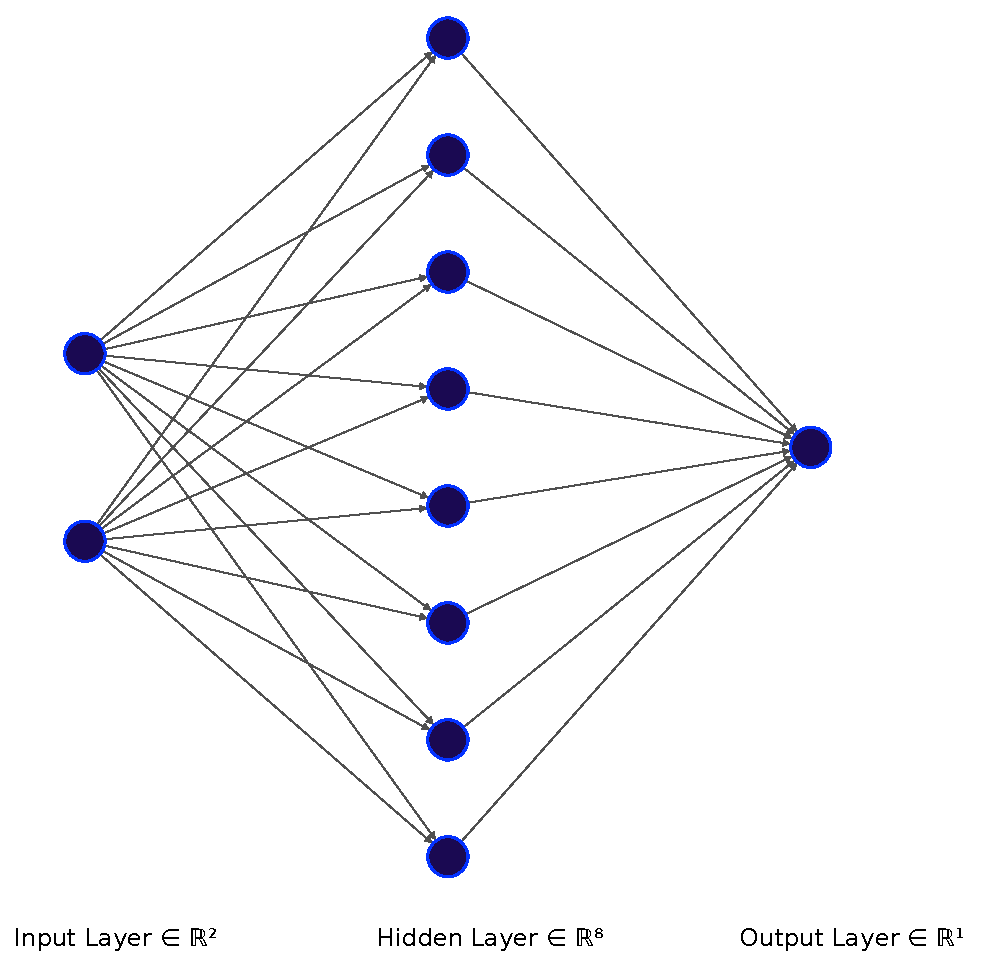
\includegraphics[width=0.45\textwidth]{nn.eps}
    \caption{Fully connected neural network with a single hidden layer}
    \label{fig:NN_single}
\end{figure}
On the other end, the Fourier series representation $S_N u$ of a T-periodic function $u$ \in $L^2(\mathbf R^M)$ is
\begin{equation}\label{Eq: fourier}
    S_{N}u(x) = \sum_{\nu \in \mathbf{N}^M, \nu_{i}\leq N} a_{\nu} \cos(\omega (\nu\cdot x)) + b_{\nu} \sin(\omega(\nu\cdot x)) 
\end{equation}
where $\omega = 2\pi/T$ and $a_{\nu}$ and $b_{\nu}$ the Fourier coefficients of $u$. It can be rewritten in the following reduced form:
 \begin{equation}\label{Eq: fourier_shift}
     S_N u(x) = \frac{a_0}{2} + \sum_{\nu \in \mathbf{N}^M, \nu_{i}\leq N} c_{\nu} \cos(\omega (\nu\cdot x) + \psi_{\nu})
 \end{equation}
where for $n \geq 1$ $c_{\nu} = \sqrt{a_{\nu}^2 + b_{\nu}^2}$ and $\psi_n = arctan2(-b_{\nu}/a_{\nu})$. In this work, we only consider the one-dimensional and leave the two-dimensional one to future work. In this case, the above expression simplifies to:

 \begin{equation}\label{Eq: fourier_shift_1d}
     S_N u(x) = \frac{a_0}{2} + \sum_{n=1}^N c_{n} \cos(n \omega x + \psi_{n})
 \end{equation}
while the output of a neural network whose goal is to approximate a 1D function becomes 
\begin{equation}\label{Eq: NN1d}
  \hat{u}(x) = \phi_0 + \sum_{k = 1}^N \lambda_{k} \sigma\left( w_{k}x + \phi_k \right),
\end{equation}
Therefore, by taking the activation function to be $\cos$ in Eq. \ref{Eq: NN1d}, one obtain a formulation equivalent to the Fourier decomposition. However as we empirically show below, the equivalency is not straightforward and one need to train the network with a specific loss function in order to obtain satisfactory results.
% Barron (\cite{Barron}) has proved that any function could be approximated by a single layer neural network with sigmoidal activation functions i.e with an activation function $\sigma$ s.t $\sigma(x) -> 0$ when $x -> -\infty$ and $\sigma(x) -> 1$ when $x -> \infty$. Leshno et al. \cite{Leshno} have proved that multilayer feedforward (define) networks with a nonpolynomial activation function can approximate any function. \\

% Here, we make use of the Fourier representation  of a T-periodic function $u$ $L^2(\mathbf R^M)$ and use the cosine function as the activation function of our network. $S_N u$ is defined as
% \begin{equation}\label{fourier}
%     S_{N}u(x) = \sum_{\nu \in \mathbf{N}^M, \nu_{i}\leq N} a_{\nu} \cos(\omega (\nu\cdot x)) + b_{\nu} \sin(\omega(\nu\cdot x)) 
% \end{equation}
% where $\omega = 2\pi/T$ and $a_{\nu}$ and $b_{\nu}$ the Fourier coefficients of $u$. In the rest of the paper, we restrict ourselves to the one-dimensional case so that the Fourier approximation is

% If we define for $n \geq 1$ $c_{\nu} = \sqrt{a_{\nu}^2 + b_{\nu}^2}$ and $\psi_n = arctan2(-b_{nu}/a_{\nu})$, we can rewrite the above decomposition as
% \begin{equation}\label{fourier_shift}
%     S_N u(x) = \frac{a_0}{2} + \sum_{\nu \in \mathbf{N}^M, \nu_{i}\leq N} c_{\nu} \cos(\omega (\nu\cdot x) + \psi_{\nu})
% \end{equation}
%\subsection{The one dimensional case}


\subsection{Loss function}
The goal of our network is to approximate the Fourier approximation $S_N u$ of $u$. To that end, we define our loss function as
 \begin{equation}\label{lossfunction}
     L(\phi, w, \lambda) = ||\hat{u} - u ||_2^2  + \alpha_1||\lambda||^2 + \alpha_2||w||^2
 \end{equation}
 where
 \begin{enumerate}
     \item The first term ensures that the output of the neural network approximates the target function $u$,
     \item The second and third terms are regularization parameters to avoid overfitting of the Neural Network. Choosing a $L^2$ norm for the regularization parameters causes the weights to decay to zero without reaching, while a $L^1$ regularization might decrease them to exactly zero. We keep the choice of the regularization for section \ref{subsec:results}.
 \end{enumerate}
 
 However, this loss function will not quite give us an approximation of the Fourier series unless we are approximating cosine or sine functions. For example, trying to fit $u(x) = x^2$ with one neuron in the hidden layer led to the output 
 $$\hat{u}(x) = \phi_0 - \lambda_1 \cos(w_1 x)$$ where  $\lambda w_1^2 /2! \approx 1$, $\lambda_1 \approx \phi_1$ and $w_1^{2l} << 1$ for $l >1$. While this, using the fact that
 $$
 \cos(w_1 x) = \sum_{l=1}^{\infty} (-1)^l\frac{w_1^{2l}x^{2l}}{(2l)!} = 1 -w_1^2x^2/2 + o(w_1^3)
 $$
 is a good approximation of $x^2$ is not the our desired result. To get the Fourier representations of our target functions, the weights from the input to the hidden layer need to be integers. This can be achieved by solving a mixed integer optimization problem which is out of the scope of this paper or by modifying the loss function as follows
  \begin{equation}\label{lossfunction_good}
     L(\phi, w, \lambda) = ||\hat{u}(x) - u(x) ||_2^2  + \alpha_1||\lambda||^2 + \alpha_2||w||^2 + \alpha_3\left( ||\hat{u}(x + T) - \hat{u}(x)||_2^2 \right)+ \alpha_4 \left( ||\hat{u}(x - T) - \hat{u}(x)||_2^2 \right)
 \end{equation}
This means we are forcing the output of the neural network to be periodic and is equivalent to the weights from the input to the hidden layer to be approximately integers.
\begin{theorem}
\textcolor{red}{need writing in terms of the nodes captured by the FNN and $S_{max of those nodes}u$}\\
Let $u$ \in $L^2(\mathbf R^M)$ be a $T$-periodic function. Then, if we denote by $\hat{u}$ the output of the constructed FNN, we have the following bounds on the approximation:
\begin{itemize}
    \item If $u$ is analytical, then $||\hat{u}(x) - u(x) ||_2^2 \le C_1 f_1(N) $ 
    \item If $u$ is piecewise analytical, then $||\hat{u}(x) - u(x) ||_2^2 \le C_2 f_2(N) $,
\end{itemize}
\end{theorem}
\begin{proof}
If $u$ is analytical, then 
$$||\hat{u}(x) - u(x) ||_2^2 \le ||\hat{u}(x) - S_N u(x) ||_2^2 + ||S_N u(x) - u(x) ||_2^2$$
\textcolor{red}{to be completed}
\end{proof}



\subsection{Weights and biases initialization}
A proper weight initialization can significantly improve the training of a neural network specially of Deep Neural Networks. In fact, when training DNNs, one is often faced with the vanishing/exploding gradients phenomenon (\cite{Geron}) which causes the training to never converge to a good solution. Here, even though we have a shallow NN, initialization is important to speed up the training. Glorot and Bengio (\cite{Glorot}) have proposed an initialization method when using the logistic activation function that circumvent that issue. In essence, they have proved that one needs the variance of the outputs of each layer should be equal the variances of its inputs. Furthermore, the variances of the gradients should be equal before and after going through a layer in the reverse direction. \cite{Heinit} proposed an initialization strategy for the $Relu$ activation function. Kumar \cite{Kumar} extended this result to nonlinear activation functions differentiable at $0$ and for the $Relu$ activation function. We propose below an initialization strategy that would make the variances equal throughout the first forward phase. As it is commonly the case, we initialize the biases to $0$. \\
Let $x$ be the input of our FNN, $\{x_k\}_{k = 1..N}$ the hidden layer nodes and $y$ the output. Then, 
$$
x_k = \cos(w_k x )
$$
and
$$
y = \sum_{k = 1}^N \lambda_k \cos(w_k x  ) 
$$
 We assume that the input $x$ is a vector of size $M$ whose elements $\{x_{j0}\}_{j0 = 1..M}$ were drawn uniformly in $[-1 \;\; 1]$. That means that $$\mu(x_{j0}) = \mu_{j0} = 0$$ and $$\sigma^2(x_{j0}) = \sigma^2_{j0} = 1/3. $$ where $\mu(z)$ denotes the mean of a random variable $z$ and $\sigma^2(z)$ its variance. 
%Therefore, the expected value of $x$ is 
% $$
% \mu(x) = [0, \cdots, 0]^T
% $$
% and  its covariance matrix
% $\Sigma(x) = $\[
%   \begin{pmatrix}
%     1/3 & 0 & \dots & 0 \\
%     0 & 1/3 & \dots & 0 \\
%     \vdots & \vdots & \ddots & \vdots \\
%     0 & 0 & \dots & 1/3
%   \end{pmatrix}
% \]


Furthermore, we assume the weights $w_k$ are drawn from a normal distribution $\mathcal N(0, w^2)$ and the weights $\lambda_k$ are drawn from a normal distribution $\mathcal N(0, v^2)$. This means $$\mu(w_k x_{j0}) = 0$$ and $$\sigma^2(w_k x_{j0}) = w^2/3.$$
We now know compute the mean of the node $k$ of the hidden layer. Using the Law of the Unconscious Statistician (LOTUS), we have:
\begin{equation}\label{muxk}
    \mu(x_k) = \int_{-1}^{1}\frac{1}{2} \int_{-\infty}^{+\infty} \cos(\pi w_k x)\frac{1}{w \sqrt{2\pi}} e^{\frac{-w_k^2}{2w^2}}\; dw_k dx 
\end{equation}
Let $I_1 = \int_{-\infty}^{+\infty} \cos(w_k x)\frac{1}{w \sqrt{2\pi}} e^{\frac{-w_k^2}{2w^2}}\; dw_k$, then
$$I_1 = \frac{|w|}{w}e^{-\frac{1}{2}w^2x^2} = e^{-\frac{1}{2}w^2x^2}. $$
This means
$$ \mu(x_k) = \int_{-1}^{1}\frac{1}{2} e^{-\frac{\pi}{2}w^2x^2} dx $$
which gives

\begin{equation}\label{muxk_last}
    \mu(x_k) = \frac{1}{w\sqrt{2\pi}}\erf\left(\frac{w\pi}{\sqrt{2}}\right) 
\end{equation}
where $\erf$ is the error function.
For the variance, we have $$\sigma^2(x_k) = \mu(x_k^2) - (\mu(x_k))^2.$$ Knowing that $$x_k^2 = \cos^2(\pi w_k x) = 1/2 + \cos(2\pi w_kx)/2,$$ we have
\begin{equation*}
    \mu(x_k^2) = \int_{-1}^{1}\frac{1}{2} \int_{-\infty}^{+\infty} \frac{1}{2}(1 + \cos(2 \pi w_k x))\frac{1}{w \sqrt{2\pi}} e^{\frac{-w_k^2}{2w^2}}\; dw_k dx
\end{equation*}
Following the same computations as above, we obtain 
$$\mu(x_k^2) = \frac{1}{2} + \frac{1}{4\sqrt{2\pi}}\frac{\erf(\sqrt{2}w\pi)}{w}$$ All in all, we therefore have
\begin{equation}\label{varxk_last}
    \sigma^2(x_k) = \frac{1}{2} + \frac{1}{4\sqrt{2\pi}}\frac{\erf(\sqrt{2}w\pi)}{w}-\left(\frac{1}{w\sqrt{2\pi}}\erf\left(\frac{w\pi}{\sqrt{2}}\right) \right)^2 .
\end{equation}
Since we want $$\sigma^2(x_k) = \frac{1}{3}, $$ we need to solve 
\begin{equation*}
    \frac{1}{3} = \frac{1}{2} + \frac{1}{4\sqrt{2\pi}}\frac{\erf(\sqrt{2}w\pi)}{w}-\left(\frac{1}{w\sqrt{2\pi}}\erf\left(\frac{w\pi}{\sqrt{2}}\right) \right)^2 .
\end{equation*}
which admits a unique solution $$w \approx 0.6959$$. However, this value being small, this means that imposing a Glorot type initialization on the hidden layer weights will cause our FNN to only capture the $0th$ and $1th$ order modes of any Fourier Decomposition(!?!). Therefore, we deliberately initialize these weights as a uniform distribution $\mathcal N(0,5)$ which means $w = \sqrt{5}$.  Plugging in this in equation (\ref{varxk_last}), we get
$$\sigma^2(x_k) = \mu(x_k^2) - (\mu(x_k))^2 \approx .5128$$. 

Now, for the output $y$, since $\lambda_k$ and $\cos(w_kx)$ are independent, we have $$\mu(y) = \sum_{k = 1}^N \mu(\lambda_k) \mu(\cos(w_k x  ))$$ and $$\sigma^2(y) = \sum_{k = 1}^N \left(\sigma^2 (\lambda_k) + \left(\mu(\lambda_k)\right)^2\right) \left(\sigma^2(\cos(w_k x  ))+\left(\mu\left(\cos(w_k x)\right)\right)^2 \right).$$ This leads to
\begin{equation}\label{vary}
    \sigma^2(y) = N\left[ v^2\left[\frac{1}{2} + \frac{1}{4\sqrt{2\pi}}\frac{\erf(\sqrt{2}w\pi)}{w}\right] \right].
\end{equation}
Since again we want $\sigma^2(y) \approx .5128$, we get 
\begin{equation}\label{varweight2}
    v^2 = \frac{0.5128}{N\left(\frac{1}{2} + \frac{1}{4\sqrt{2\pi}}\frac{\erf(\sqrt{2}w\pi)}{w}\right)} 
\end{equation}
where $w = \sqrt{5}$.




\subsection{Results}\label{subsec:results}
 \begin{table}[!h]
  \begin{center}
\begin{tabular}{ |c|c|c|c|c| } 
\hline
$w_k$ & $\phi_k$ & $\lambda_k$& $\phi_0$ \\
\hline
$1.00000000$ & $-0.78539816 \approx -\pi/4$ &$1.41421354 \approx \sqrt{2}$& \\ 
$-5.96856597e-07$&$-1.00911547$ & $-2.60499122e-05$& $-1.81893539e-05$ \\ 
$1.22755482e-06$& $1.87773726$ & $-4.76966579e-05$& \\ 
$4.59348246e-08$& $-6.38405893 $ & $1.77429347e-05$& \\ 
\hline
\end{tabular}
\caption{Optimal weights and biases of the FNN to approximate $ f(x) = \cos(\pi x) + \sin(\pi x)$, $k = 1\cdots4$ with a $L^2$ regularization. Optimization converged after $189$ iterations.}\label{tabcossinL2}
\end{center}
\end{table}

\subsubsection{Analytical Periodic Functions}
 \begin{table}[!h]
  \begin{center}
\begin{tabular}{ |c|c|c|c|c| } 
\hline
$w_k$ & $\phi_k$ & $\lambda_k$& $\phi_0$ \\
\hline
$1.00000033$ & $-0.78540193 \approx -\pi/4$ &$1.41421847 \approx \sqrt{2}$& \\ 
$1.4969094$&$-0.71483098$ & $-4.32639025e-06$& $1.58219741e-05$ \\ 
$0.05095418$& $ 0.96613253$ & $6.73308554e-05$& \\ 
$0.14126515$& $-5.84166681 $ & $-5.13186621e-05$& \\ 
\hline
\end{tabular}
\caption{Optimal weights and biases of the FNN to approximate $ f(x) = \cos(\pi x) + \sin(\pi x)$, $k = 1\cdots4$ with a $L^1$ regularization. Optimization converged after $87$ iterations.}\label{tabcossinL1}
\end{center}
\end{table}
We first tried to approximate the 2-periodic function 
 $$
 f(x) = \cos(\pi x) + \sin(\pi x)\;.
 $$
 with a neural network comprised of four nodes in the hidden layer. We show results for both $L^2$ and $L^1$ weights regularizations.
From tables (\ref{tabcossinL2}-\ref{tabcossinL1}) we can see that the output of the FNN is $\hat{u}(x) \approx \sqrt{2}\cos(\pi x - \frac{\pi}{4})$ which is the reduced form of  $f(x)= \cos(\pi x) + \sin(\pi x)$ for both $L^2$ and $L^1$ regularizations. The optimization converged to approximately $2e-4$ in $189$ iterations for the $L^2$ regularization against $3e-4$ in $87$ iterations for the $L^1$ one. Although the results for the $L^1$ are slightly better, one would expect the hidden layer to output weights to be exactly zero for all but one of the nodes.

We compare in figure (\ref{fig:fourvsNN_iter}) the convergence of the optimization between the FNN with $L^1$ and $L^2$ regularization to the convergence of a regular neural network with a $\tanh$ activation function and a Glorot initialization. The latter network converged to approximately $1e-3$ in $1173$ iterations which showcases the gain in iteration number and accuracy we obtain using a FNN for the class of functions on interest in this section.

%  \begin{figure}[!htb]
%     \centering
%     \subfigure{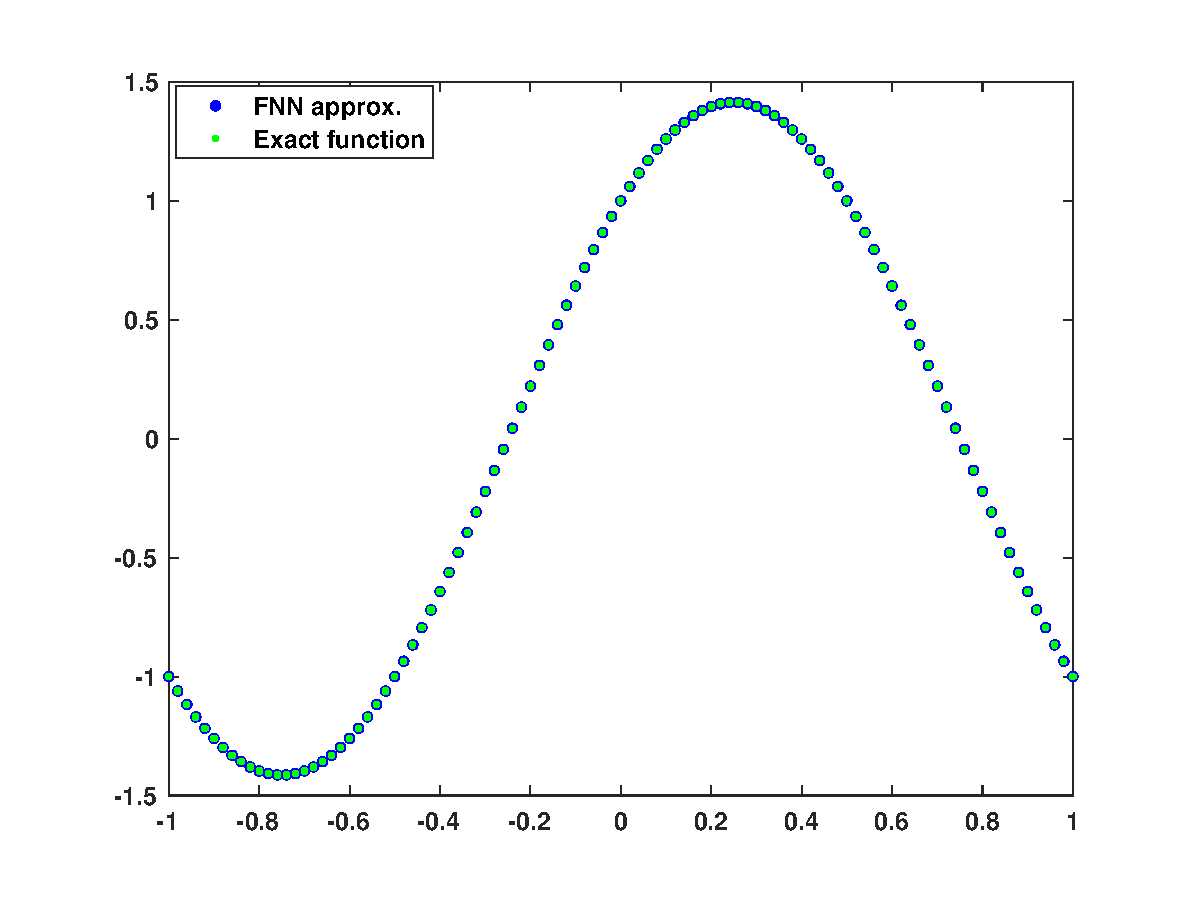
\includegraphics[width=0.45\textwidth]{FNNcossinnodes4.eps}}
%     \subfigure{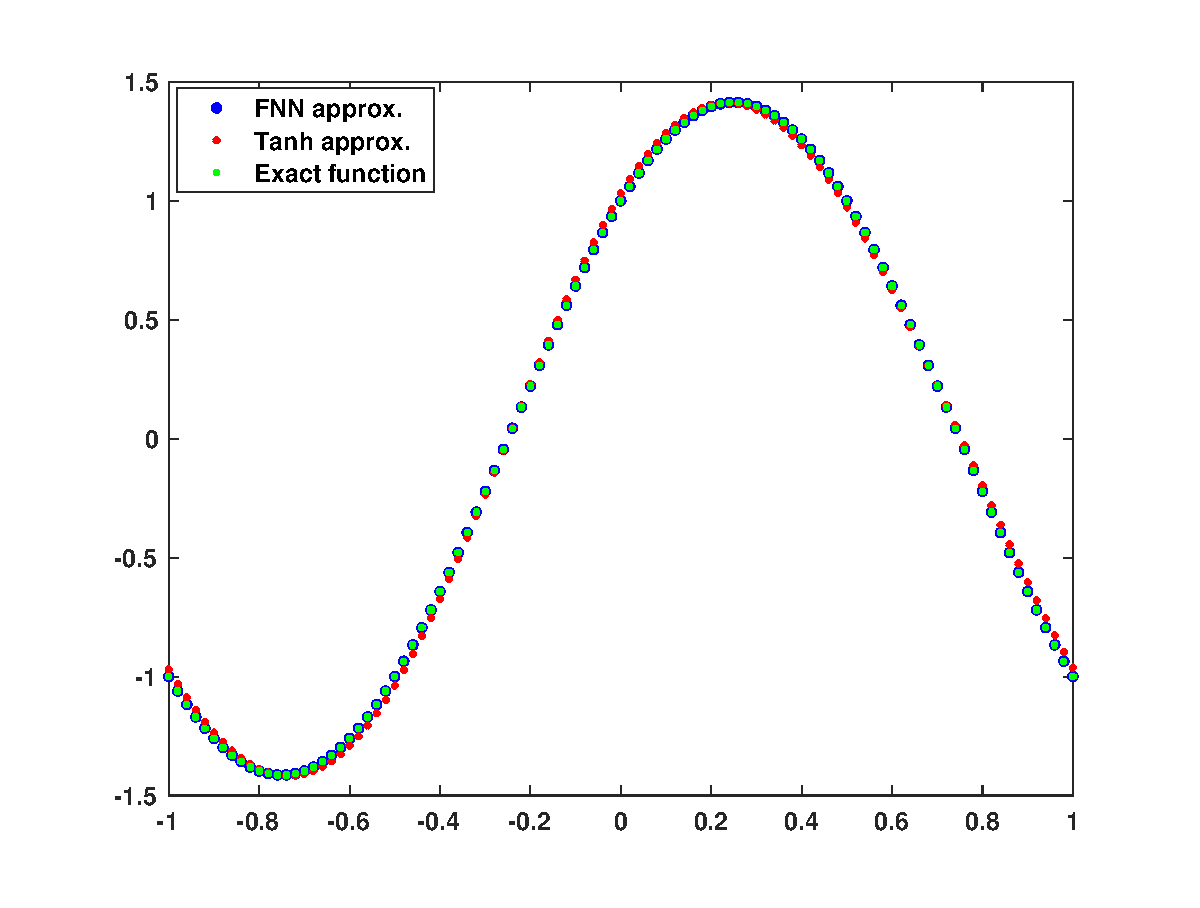
\includegraphics[width=0.45\textwidth]{FNNvstanhsincos.eps}}
%     \caption{(Top)Comparison between the approximation obtained by our Fourier Neural Network and the exact solution. (Bottom)Comparison between the approximation obtained by using a tanh activation function and the exact solution}
%     \label{fig:fourvsNN_percs}
% \end{figure}

 \begin{figure}[!htb]
    \centering
    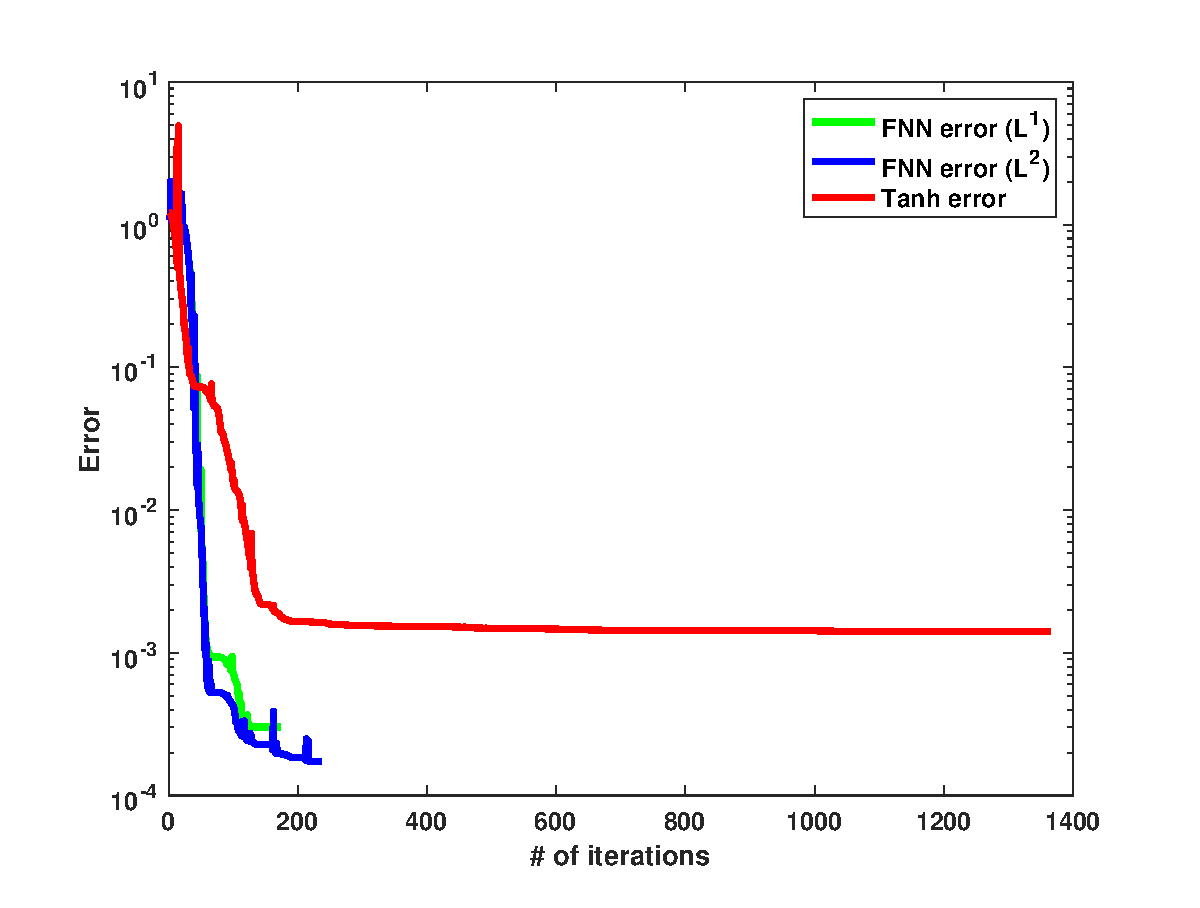
\includegraphics[width=0.8\textwidth]{itertanhvsfnn.eps}
    \caption{(Top)Comparison in terms of iteration number and error between using a FNN and using a neural network with a $\tanh$ activation.}
    \label{fig:fourvsNN_iter}
\end{figure}
 Furthermore, as shown in figure (\ref{fig:fourvsNN_outside}), a big advantage of our neural network is that it remains a good approximation outside of the training domain which is rarely the case when using neural networks.
   \begin{figure}[!htb]
    \centering
    \subfigure{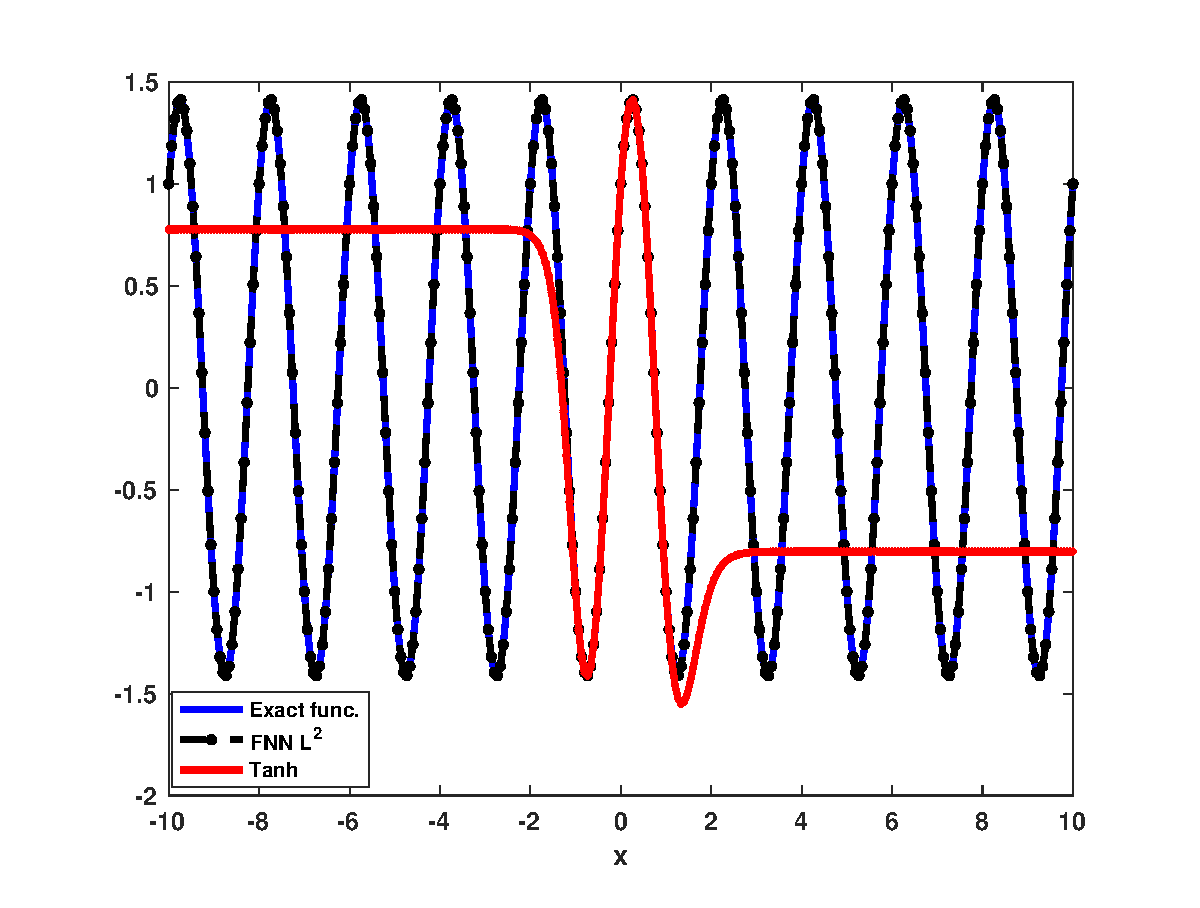
\includegraphics[width=0.7\textwidth]{fnnl2vstanhoutside.eps}}
     \subfigure{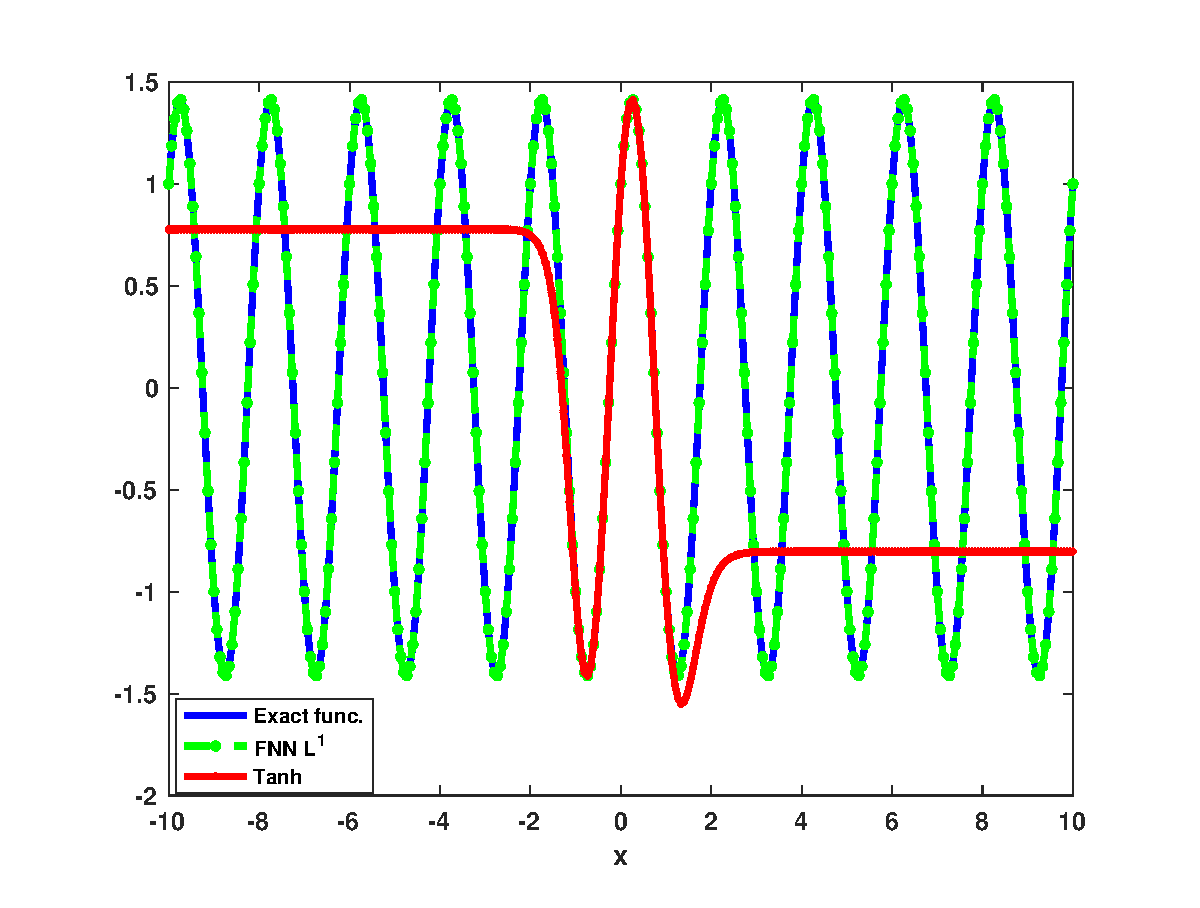
\includegraphics[width=0.7\textwidth]{fnnl1vstanhoutside.eps}}
    \caption{Comparison outside of the training domain for both $L^2$ (top) and $L^1$ regularizations}
    \label{fig:fourvsNN_outside}
\end{figure}


We then tried to approximate the function 
$$g(x) = 8 \cos(4\pi x) + \sin(2\pi x) + \sin(\pi x)$$ with the same architecture as above. The optimization converged to approximately $9e-4$ after $195$ iterations when using a $L^2$ regularization on the weights and to approximately $1e-3$ after $169$ iterations when using a $L^1$ one. We show in tables (\ref{tabpercompL2}-\ref{\tabpercompL1}) the values of the weights obtained at convergence. We see the biases approximating odd multiples of $\pi/2$ for the $\sin$ part of the function we are approximating. 

%tanh converged to 3e-2 in 2049 it with 10 nodes
 \begin{table}[!h]
  \begin{center}
  \begin{tabular}{ |c|c|c|c|c| } 
\hline
$w_k$ & $\phi_k$ & $\lambda_k$& $\phi_0$ \\
\hline
$1.00000000$ & $1.57079627 \approx \pi/2$ &$-9.99999993e-01$& \\ 
$5.40604942e-06$&$1.01888743e+01$ & $3.34351764e-06$& $2.41330937e-06$ \\ 
$4.00000000$& $-9.14402304e-10$ & $7.99999983$& \\ 
$ -2.00000000$& $4.71238899 \approx 3\pi/2$ & $-9.99999984e-01$& \\ 
\hline
\end{tabular}
\caption{Optimal weights and biases of the FNN to approximate $ g(x) = 8 \cos(4\pi x) + \sin(2\pi x) + \sin(\pi x)$ with $L^2$ regularization, $k = 1\cdots4$, converged to $9e-4$ 195 ite}\label{tabpercompL2}
\end{center}
\end{table}


 \begin{table}[!h]
  \begin{center}
  \begin{tabular}{ |c|c|c|c|c| } 
\hline
$w_k$ & $\phi_k$ & $\lambda_k$& $\phi_0$ \\
\hline
$0.99999306$ & $1.57072838 \approx \pi/2$ &$-1.000141261$& \\ 
$1.99999672$&$7.85406634 \approx 5\pi/2$ & $-9.99825909e-01$& $3.82384745e-05$ \\ 
$3.99999998$& $-1.14376588e-05$ & $7.99989569$& \\ 
$ -0.04032155$& $-2.12089270e+01$ & $1.69927207e-05$& \\ 
\hline
\end{tabular}
\caption{Optimal weights and biases of the FNN to approximate $ g(x) = 8 \cos(4\pi x) + \sin(2\pi x) + \sin(\pi x)$ with $L^1$ regularization, $k = 1\cdots4$, converged to $1e-3$ 169 ite}\label{tabpercompL1}
\end{center}
\end{table}
We show in figure (\ref{fig:fourvsNNcompPer}) a comparison between the exact function and the approximations of our FNN. The actual error between only the function and the FNN approximation is of the order of $1e-8$ for the $L^2$ regularization and $1e-5$ for the $L^1$ one. For this reason, we use only $L^2$ regularization in the rest of the paper. Furthermore, a regular neural network with a $\tanh$ activation converged to a poor local minimum for $4$ nodes in the hidden layer. It converged to an acceptable error of $3e-2$ for $10$ nodes. Therefore, our FNN is noticeably superior for this function. (\textcolor{red}{should I add comparison?})
 \begin{figure}[!htb]
    \centering
    \subfigure{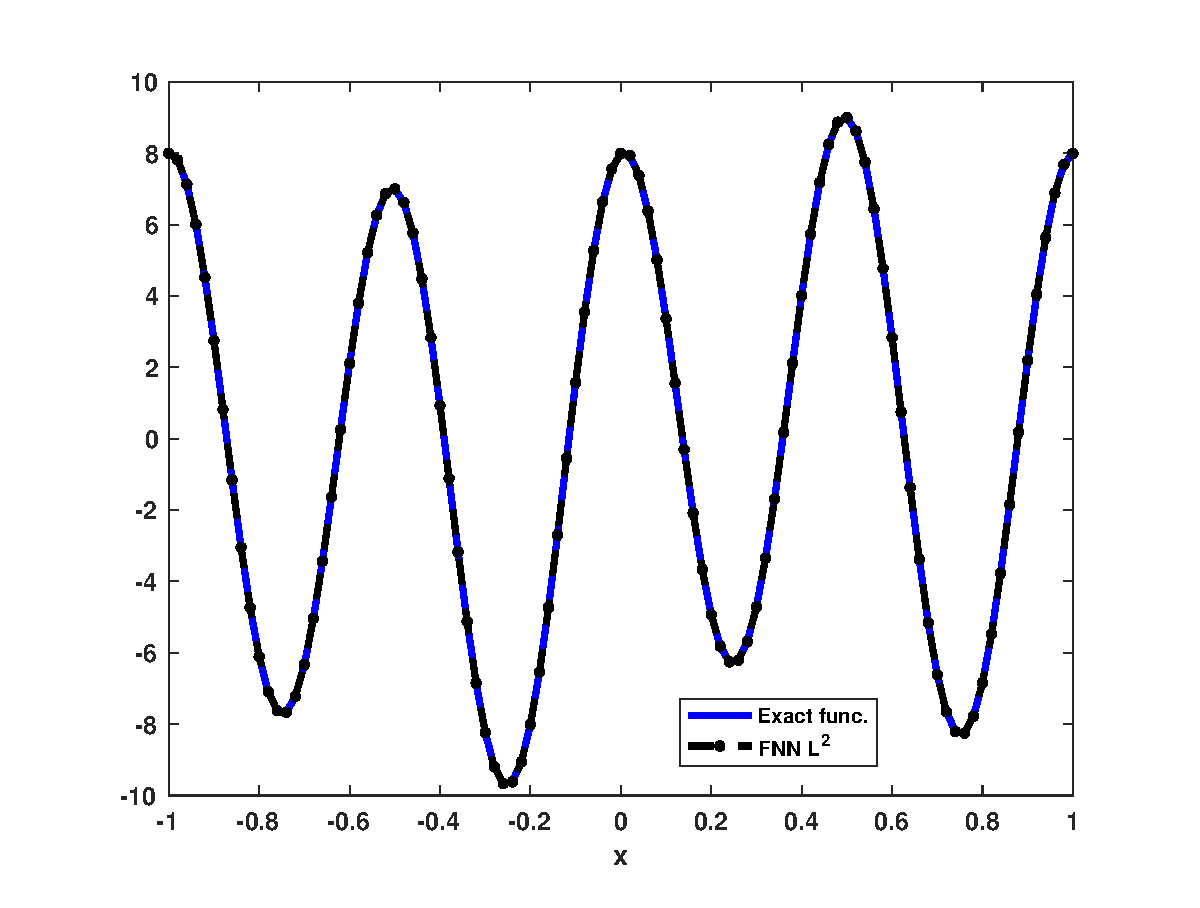
\includegraphics[width=0.7\textwidth]{fnnl2vsexactcomp.eps}}
     \subfigure{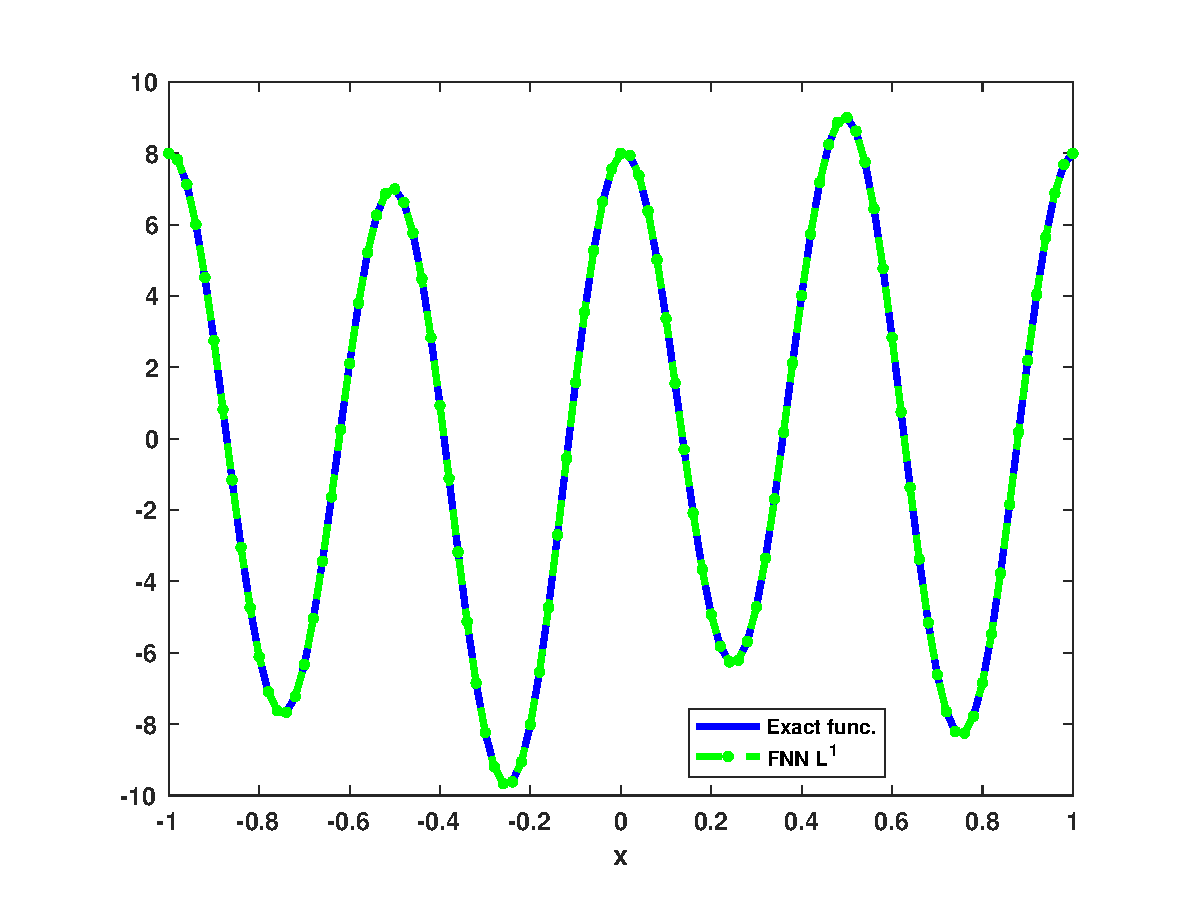
\includegraphics[width=0.7\textwidth]{fnnl1vsexactcomp.eps}}
    \caption{Comparison between $g(x) = 8 \cos(4\pi x) + \sin(2\pi x) + \sin(\pi x)$ and the output of the FNN for both $L^2$ (top) and $L^1$ regularizations}
    \label{fig:fourvsNN_outside}
\end{figure}



\subsubsection{Continuous periodic functions}  
Here, we first tried to approximate the non analytical periodic function
$$
f(x) = x^2, \;\; \text{$x \in \left(-(2k+1), (2k+1)\right)$}\;\;, k \in \mathbf{N}
$$
The Fourier series of this function is
$$
S(f)(x)= \frac{1}{3} + \sum_{n=1}^{\infty} 4 \frac{(-1)^n}{\pi^2 n^2} \cos(\pi nx)
$$
We used again $4$ nodes in the hidden layer and the FNN captured the first $5$ nodes of the Fourier decomposition (if we count the $0th$ node). We show in table (\ref{tabfnnx2}) the values obtained for the weights and the biases. Calling FNN coefficients the hidden layer to output layer supplemented by the output layer's bias (the $0th$ node), we see that they are $3rd$ order approximations of the actual Fourier coefficients. Figure (\ref{Fnnx2}) is a good visual of the quality of that approximation.
\begin{table}[!h]
  \begin{center}
  \begin{tabular}{ |c|c|c|c|c| } 
\hline
$w_k$ & $\phi_k$ & $\lambda_k$& $\phi_0$ \\
\hline
$0.99995578$ & $-0.00477923$ &$-0.40479907$& \\ 
$2.99892898$&$-3.139197051$ & $0.04915202$& $0.335023246$ \\ 
$3.99604127$& $0.01794715$ & $0.02874206$& \\ 
$ -1.99965386$& $0.00445702$ & $ 0.10497063$& \\ 
\hline
\end{tabular}
\caption{Optimal weights and biases of the FNN to approximate $ f(x) = x^2$ on $[-1, 1$]}\label{tabfnnx2}
\end{center}
\end{table}

  \begin{figure}[!htb]
    \centering
    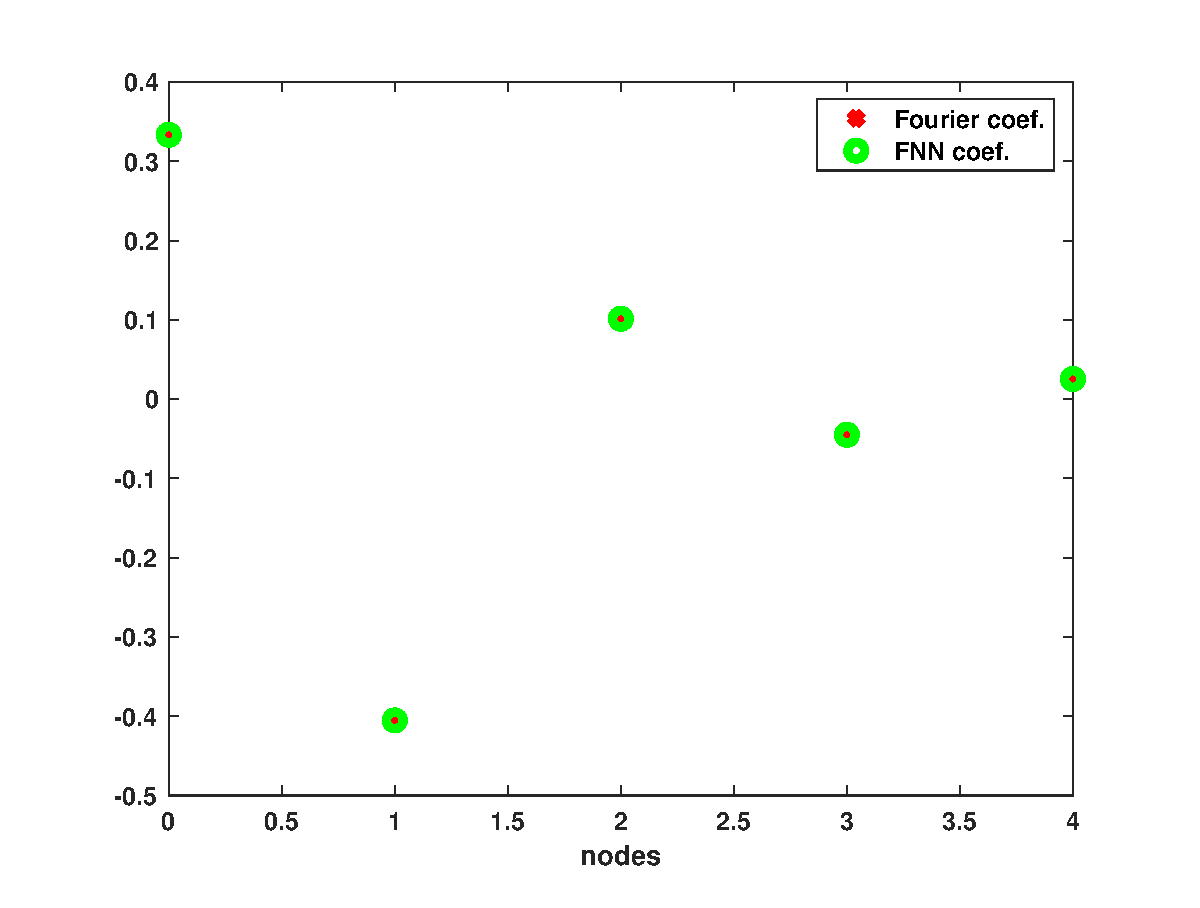
\includegraphics[width=.8\textwidth]{fnncoeffvsfourcoef.eps}
    \caption{Comparison between the FNN coefficients and the Fourier coefficients for the $4$ nodes captured by the neural network}
    \label{Fnnx2}
\end{figure}
We also showcase in figure (\ref{Fnnx2out}) the behavior of the output of the FNN as opposed to the one from a $tanh$ neural network. As expected, our network conserves the  properties of the function to be approximated outside of the training domain while the $tanh$ neural network does not. It is worth noticing that the latter was more accurate in this case on the training interval $[-1, 1]$ ($6e-4$ with $3073$ iterations against $2e-2$ with $130$ iterations.)
\begin{figure}[!htb]
    \centering
    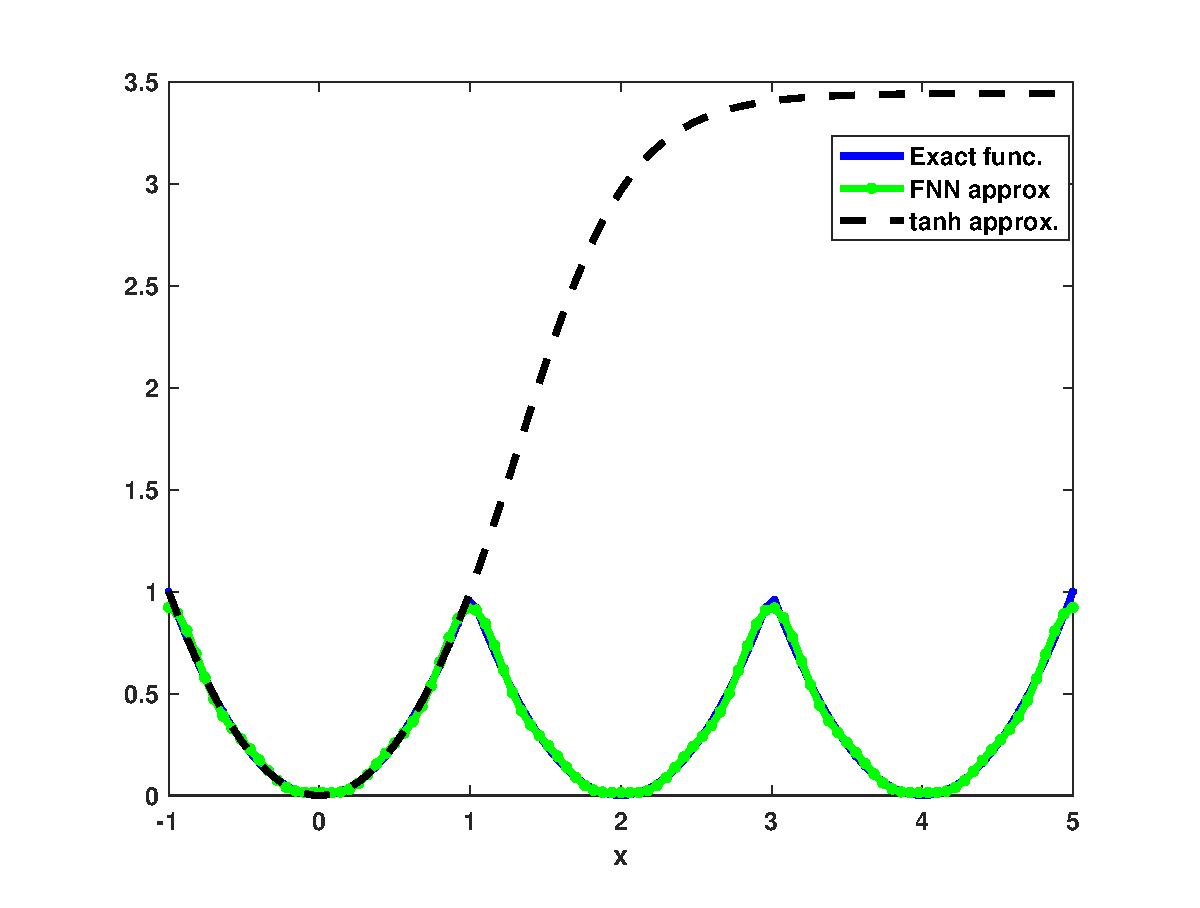
\includegraphics[width=.8\textwidth]{fnnvstanhoutx2.eps}
    \caption{Comparison between the FNN and the $\tanh$ approximations outside the training domain}
    \label{Fnnx2out}
\end{figure}


We also approximated the function
$$
g(x) = |x|, \;\; \text{$x \in \left(-(2k+1), (2k+1)\right)$}\;\;, k \in \mathbf{N}
$$
The Fourier series of this function is
$$
S(g)(x)= \frac{1}{2} + \sum_{n=1}^{\infty} -4 \frac{(1}{\pi^2 (2n - 1)} \cos(\pi (2n - 1)x)
$$
We summarize in table (\ref{tabfnnx2}) the FNN coefficients as well as the biases. Here, the FNN captured the first $4$ nodes of the Fourier decomposition. This can be explained by the fact $g$ only admits odd nodes. As before, we give a visual comparing the Fourier coefficients of $g$ to the FNN coefficients in figure (\ref{Fnnabsx}). Here again, the FNN coefficients are good approximations of their Fourier counterparts. The error between the two is again of the $3rd$ order.\\


\begin{table}[!h]
  \begin{center}
  \begin{tabular}{ |c|c|c|c|c| } 
\hline
$w_k$ & $\phi_k$ & $\lambda_k$& $\phi_0$ \\
\hline
$ 0.99995402$ & $-2.44738021e-03$ &$-0.40420162$& \\ 
$2.98845687$&$-1.68031025e-01$ & $0.03295792$& $0.502531$ \\ 
$2.99445216$& $-6.78306499e-02$ & $-0.07711458$& \\ 
$ -1.99075052$& $-9.45244148$ & $ -0.00391551$& \\ 
\hline
\end{tabular}
\caption{Optimal weights and biases of the FNN to approximate $ f(x) = |x|$ on $[-1, 1$]}\label{tabfnnx2}
\end{center}
\end{table}

  \begin{figure}[!htb]
    \centering
    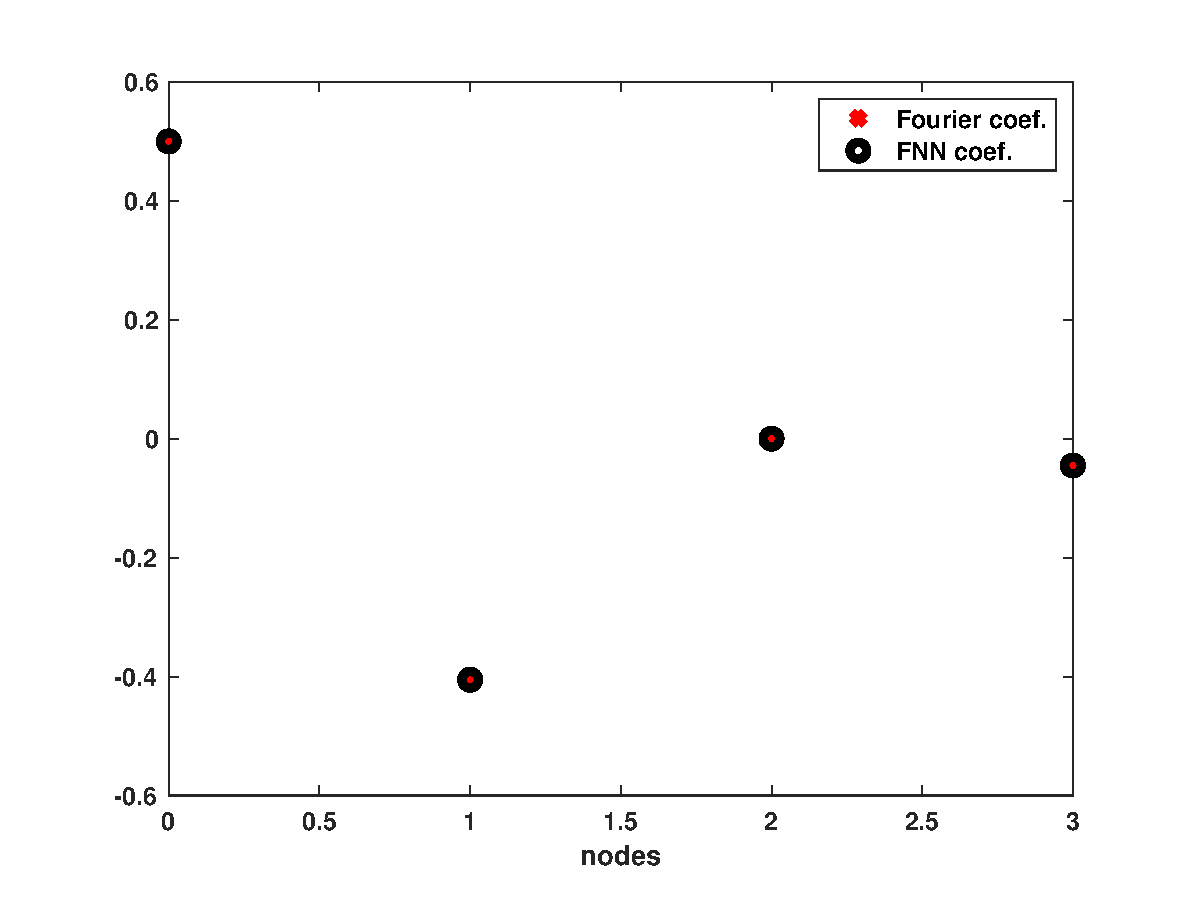
\includegraphics[width=.8\textwidth]{fnncoeffvsfourcoeffabsx.eps}
    \caption{Comparison between the FNN coefficients and the Fourier coefficients for the $4$ nodes captured by the neural network}
    \label{Fnnabsx}
\end{figure}







\section{Fourier neural networks as differential equations solvers}
\textcolor{red}{Needs reruns since you changed initialization strategy}
In this section, we are seeking periodic solutions of differential equations of the type $$Nu = f$$ where $N$ is a differential operator. The construction of a Fourier neural network that acts as a differential solver is the same as above with only the loss function changing. Following \cite{Sirignano} and \cite{Raissi}, we use
\begin{equation}\label{lossfunPDE}
     L(\phi, w, \lambda) = ||N \hat{u}(x) - f(x) ||^2  + \alpha_2||\lambda||^2 + \alpha_3||w||^2 + \alpha_3\left( ||\hat{u}(x + T) - \hat{u}(x)||^2\right) + \alpha_4\left( ||\hat{u}(x - T) - \hat{u}(x)||^2 \right)
\end{equation}
that incorporates the physics into the loss function to obtain what we call a physics informed Fourier neural network. 

First, we solve the Poisson Equation
\begin{equation}\label{Poisson}
    -\Delta u = \cos(\pi x),\;\;\; x \in [-1,1].
\end{equation}
with the constructed FNN. Tto assess the quality of the FNN solution, we can compare it to the exact solution of this equation which is given by $u = 1/(\pi^2)\cos(\pi x)$.
  \begin{figure}[!htb]
    \centering
    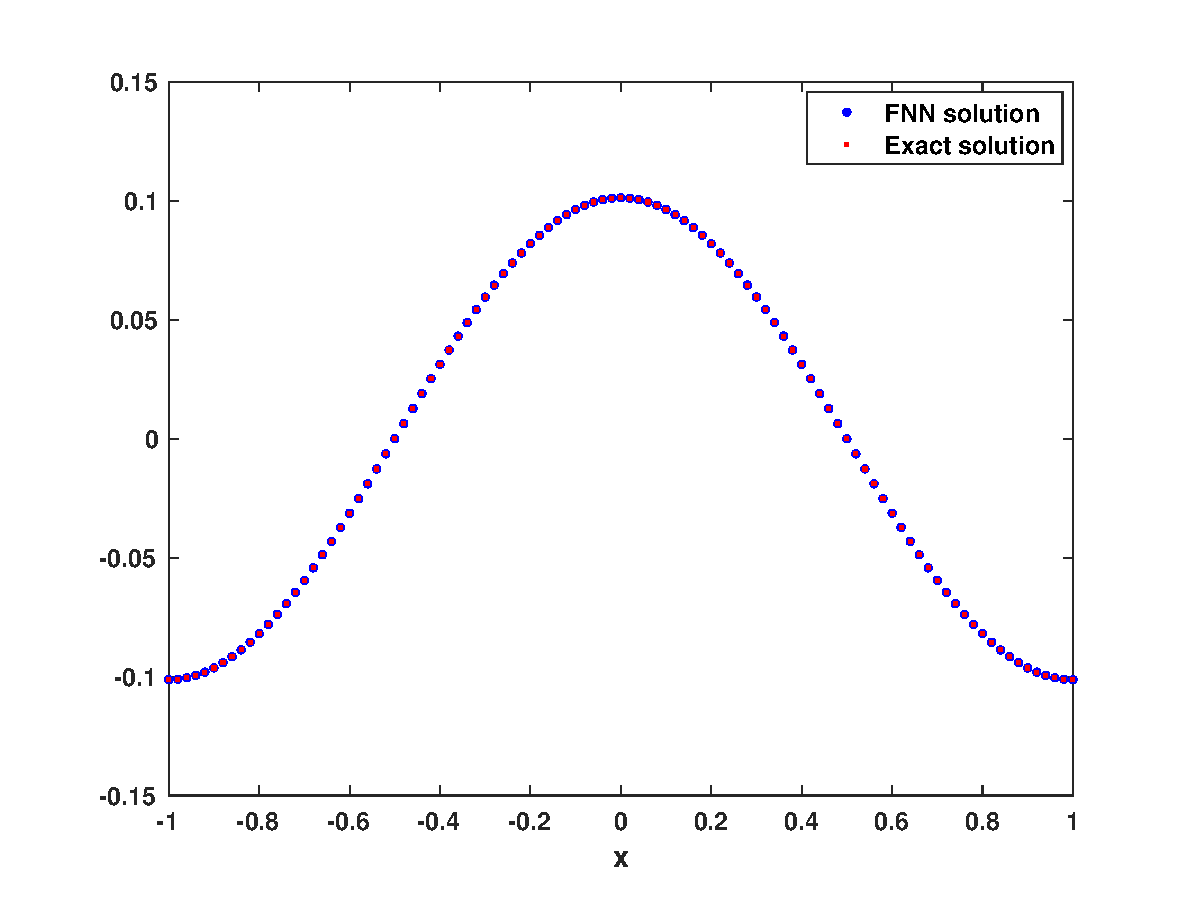
\includegraphics[width=.8\textwidth]{FNNvsexPoisson1d.eps}
    \caption{Comparison between the FNN and the exact solutions}
    \label{fig:FNNvsexactPoisson}
\end{figure}
In figure (\ref{fig:FNNvsexactPoisson}) we see that the solution obtained by the FNN is a good approximation of the exact one. The order of the relative error between the two is $1e-6$.\\

We then solve the heat equation \textcolor{red}{Put in align mode}
\begin{equation}\label{Heat}
    \frac{\partial u}{\partial t} = \frac{\partial^2 u}{\partial^2 x},\; x \in [-1,1] \;\;\; u(0,x) = u_0(x) = 6 \sin(\pi x), \;\;\; u(t, -1) = u(t, 1).
\end{equation}
To account of the time dependency, we rewrite the heat equation using separation of variables method. To that end, we set $u(x,t) = X(x)T(t)$ which transforms the equation into 
$$X(x)T'(t) = X''(x)T(t).$$
We rewrite the cost function as follows 
\begin{align*}
    L(\phi, w, \lambda) &= \alpha_1||\hat{X}(x)\hat{T}'(t)-\hat{X}''(x)\hat{T}(t)||^2  \\ &+\alpha_2||\lambda||^2 + \alpha_3||w||^2 \\ 
    &+\alpha_3 ||\hat{X}(x + 2) - \hat{X}(x)||^2 \\
    &+\alpha_4||\hat{X}(x - 2) - \hat{X}(x)||^2  \\
   &+ \alpha_5||\hat{T}_0(x) - \hat{u}_0(x)||^2
\end{align*}
Since the solution of Eq. (\ref{Heat}) is separable, we separate our network into two independant subnetworks. One with the FNN architecture and one with a regular architecture (with a $\tanh$ activation function.) \textcolor{red}{PUT figure of architecture here.}


  \begin{figure}[!htb]
    \centering
    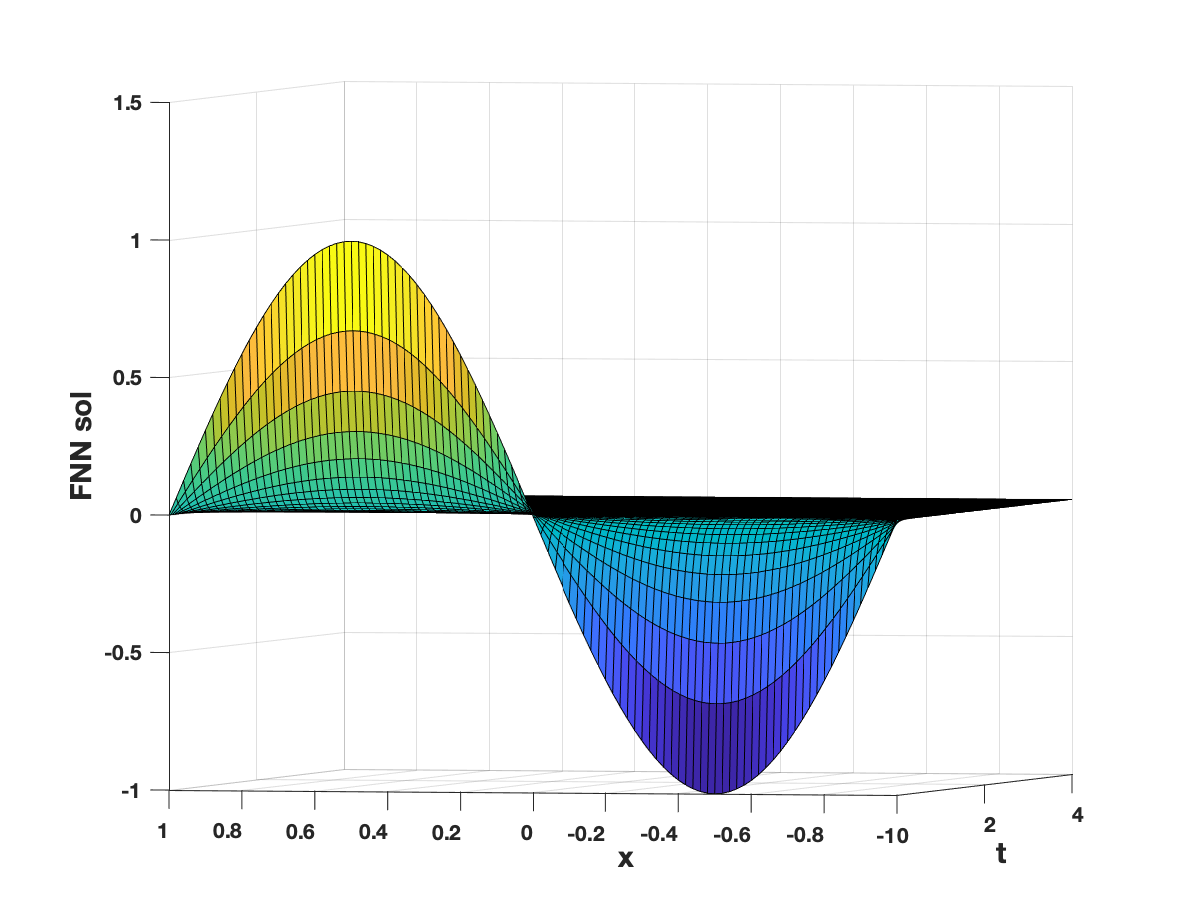
\includegraphics[width=.8\textwidth]{NNheatsol.eps}
    \caption{Comparison between the FNN and the exact solutions}
    \label{fig:fourvsNNcompPer}
\end{figure}

Finally, we solve the following system of differential equations obtained from \cite{Teschl2012} 
\begin{align}
    \frac{\partial x_1}{\partial t} &= -\pi  x_2 + x_1(1 - x_1^2 - x_2^2) \nonumber \\ 
    \frac{\partial x_2}{\partial t} &= \pi  x_1 + x_2(1 - x_1^2 - x_2^2) \\
\end{align}\label{sys_per}
This system admits a periodic solution given by $u(t)=(cos(\pi t), sin(\pi t))$


%\section{Results}



\section{Conclusion}

























\bibliographystyle{plain}
\bibliography{bie}
\end{document}

%  which looks like the Fourier series of $u$. Hence the goal of our network is to find weights $w$ and biases $\phi$ that equate the fourier coefficients $c_n$ and phase shift $\psi_n$. Obviously, for trigonometric functions, one would need a fewer nodes in the hidden layer than for other functions. For example, one would expect our neural network to converge to the solution quickly if the function to be learned is $\cos(x)$ and to only need one neuron in the hidden layer. To avoid using too many or too few neurons in the hidden layer,  we use a dynamical approach. We start with a hidden layer with one neuron and add neurons as the optimization unfold.



% \subsection{The multidimensional case}
% In order to approximate equation (\ref{fourier_shift}), we construct the network with $M$ inputs and write the output as
% $$ \hat{u}(x) = \phi_0 + \sum_{k = 1}^N \lambda_k \cos\left( w_k\cdot x + \phi_k. \right)$$
% and use the same loss function as before. In this case, one need more neurons in the hidden layer in order to skip less $\nu$ in equation \ref{fourier_shift} as possible.



%  \subsection{Results}
%  In order to retrieve the Fourier series of $u$, we train our neural network with the loss function
%  \begin{equation}\label{loss}
%     L(\phi, w, \lambda) = \sum_{k = 1}^N |\hat{u}(x_k) - u(x_k)|^2
%  \end{equation}
% where $\{x_k\}_{k=1}^{N}$ is the training data that is uniformly drawn in $[\pi/2, \pi/2]$

% To validate the model, we first try to recover $u: x -> \cos(x)$ with one neuron in the hidden layer and compare the results with a network trained with the sigmoid and hyperbolic tangent functions. 
% Our neural network converges after $85$ iterations and give $$\hat{u}(x) = -\cos(-x + 3.14159265 ) + -1.29629469e-17 \approx -\cos(-x + \pi) = \cos(x) $$.
% Using the sigmoid function with $N = 10$ nodes converged in $3516$ iterations and hyperbolic tangent in $2696$ iterations. Furthermore, using a cosine activation function with a Xavier intialization, converges to a loss value of $.68$ which is quite big(\textbf{Put it in a table}).




% Then, we try to fit the periodic $u: x -> x^2$ on $[-\pi, \pi]$



% \textbf(Multiple hidden layers: First one uses sin/cos activation functions, following uses Relu/sigmoid etc?)
% \textbf(Make us of convolutions?)
% \textbf(Use Differentiation matrices?(Chebyshev))


% The goal of this work is to learn periodic solutions of partial differential equations using a Fourier based Neural Network. More specifically, we will use a neural network with one hidden layer and with an activation function in the form of Fourier basis. We then compare our results to the one obtained from neural networks using sigmoid and reLU activation functions.

% PUT FIGURE OF NN WITH FOURIER BASIS AND SHOW HOW THEY APPROXIMATE ANY L2 PERIODIC  FUNCTION

% \textbf{Tentative Algorithm}
% \begin{itemize}
% \item First, compress the data using DCT plus mode selections
% \item Second, Use Chebychev Differentiation matrices
% \item Third, Apply ML

% \end{itemize}



%\subsection{Weights and biases initialization}




%   It is common practice to initialize the biases of a neural network at $0$ and the weights using a Xavier initialization (\cite{Glorot}) or a He initialization (\cite{Heinit}). \cite{Kumar} also proposed a weight initialization for activation functions differentiable at zero or not but with biases initialized at zero. When initializing the weights of a neural network, one would like to have $$var(x_{i+1}) = \sigma_{i+1}^2 = var(x_{i}) = \sigma_{i}^2$$. Here we initialize the biases ${\phi_i}_{i=0}^{N}$ uniformly on $[\pi/2, pi/2]$ i.e $\phi_i~ U([-pi/2, pi/2])$. That means the expectation $\mu(\phi_i) = 0$ and $var(\phi_i) = 1/12$. We also suppose that the inputs ${x_0(j)}_{j=1}^M$ are uniformly drawn on $[-\pi, \pi]$. Thetrefore, $\mu(x_j) = 0$ and $var(x_0(j)) = \sigma_i = 1/3.$ Additionnaly, we assume the weights $\lambda_{kj}$ are drawn from a normal distribution with mean $0$ and variance $v^2$ and the $w_k$ from a normal distribution with mean $0$ and variance $\omega^2$. The goal is to find $v^2$ and $\omega^2$ s.t $$var(x_{i+1}) = \sigma_{i+1}^2 = var(x_{i}) = \sigma_{i}^2$$.\\
 
%   From the form of our network, we have for the neurons in the hidden layer and using Taylor approximations, we have
%   \begin{equation}
%       x_1{i} \approx \cos(\phi^1_i) + y_0(1)(-\sin(\phi^1_i))
%   \end{equation}
%   where $y_0(1) = \sum_{j=1}^M \lambda_{1j}x_0(j)$. From this, we have $\mu(y_0(1)) = 0$ and $var(y_0(1)) = M* v^2 * pi^2/3$.
%   Therefore, $\mu(x_1{i}) = \mu(\cos(\phi^1_i))$. Using the law of the unconscious statistician, we have 
%   \begin{align*}
%       \mu_1 = \mu(x_1(i)) = \mu(\cos(\phi^1_i)) &= \int_{0}^{\pi/2} \frac{1}{\pi}\cos(\phi^1_i)  + \int_{-\pi/2}^{0} -\frac{1}{\pi}\cos(-\phi^1_i)\\
%       &= \int_{0}^{\pi/2} \frac{1}{\pi}\cos(\phi^1_i)  + \int_{0}^{\pi/2} \frac{1}{\pi}\cos(-\phi^1_i)\\
%       &= \int_{0}^{\pi/2} \frac{1}{\pi}\cos(\phi^1_i)  + \int_{0}^{\pi/2} \frac{1}{\pi}\cos(\phi^1_i)\\
%       &= 2\int_{0}^{\pi/2} \frac{1}{\pi}\cos(\phi^1_i) \\
%       &=  \frac{2}{\pi}
%   \end{align*}
%   where we have used the fact that $\cos(-x) = cos(x)$.
%   For the variance, we have
%   \begin{align*}
%       s_1^2 = var(\cos(\phi^1_i)) + \mu(y_0^2(i))\mu(\sin^2(\phi^1_i)) - \mu(y_0^(i))^2\mu(\sin(\phi^1_i))^2
%   \end{align*}
%   We use again the law of the unconscious statistician and obtain
%   \begin{align*}
%       \mu(\sin^2(\phi^1_i)) = \mu(1 - \cos^2(\phi^1_i)) = 1 - \mu(\sin^2(\phi^1_i)) = 1 -1/2 = 1/2
%   \end{align*}
%   Therefore,
%   \begin{align*}
%       s_1^2 = 1/2 - (2/pi)^2 + M* v^2 * pi^2/6
%   \end{align*}
%   We want $s_1^2 = 1/3$ so, we have the following equation for $v^2$
%   \begin{equation*}
%       1/3 = 1/2 - (2/pi)^2 + M* v^2 * pi^2/6
%   \end{equation*}
%   which means
%   \begin{equation}
%       v^2 = \frac{6}{M1}\left(1/3 - 1/2 +4/1 \right)
%   \end{equation}
%   Now, for the output, we have
%   \begin{equation*}
%       x_2 = \sum_{i =1}^N w_i x_1(i) + \phi_0
%   \end{equation*}
%   So that 
%   \begin{align*}
%       \mu(x_2) &= \sum_{i =1}^N \mu(w_i) \mu(x_1(i)) + \mu(\phi_0) \\
%           &= \mu(\phi_0) = 0
%   \end{align*}
%   and
%   \begin{align*}
%       s_2^2 &= \sum_{i =1}^N \left(\mu(w_i^2) \mu(x_1^2(i))-  \mu^2(w_i) \mu^2(x_1(i))\right) + var(\phi_0) \\
%           &= N\omega^2(s_1^2 - \mu_1^2) + var(\phi_0)\\
%           & = N\omega^2(\frac{1}{3} - \frac{4}{1}) + var(\phi_0)
%   \end{align*}
%   Again, we want $s_2^2 = \frac{pi^2}{3}$. To achieve that, we initialize the output bias at $0$ so that $var(\phi_0) = 0$ and set
%   \begin{equation}
%       \omega^2 = \frac{1}{3N(1/3 - 4/1)}
%   \end{equation}


%%%%%%%%
% Next, we tried a more complicated $2\pi$-periodic function
%  $$
%  f(x) = 2\cos(10x) + \sin(7x) + + \sin(2x)
%  $$
%  \begin{figure}[!htb]
%     \centering
%     \subfigure{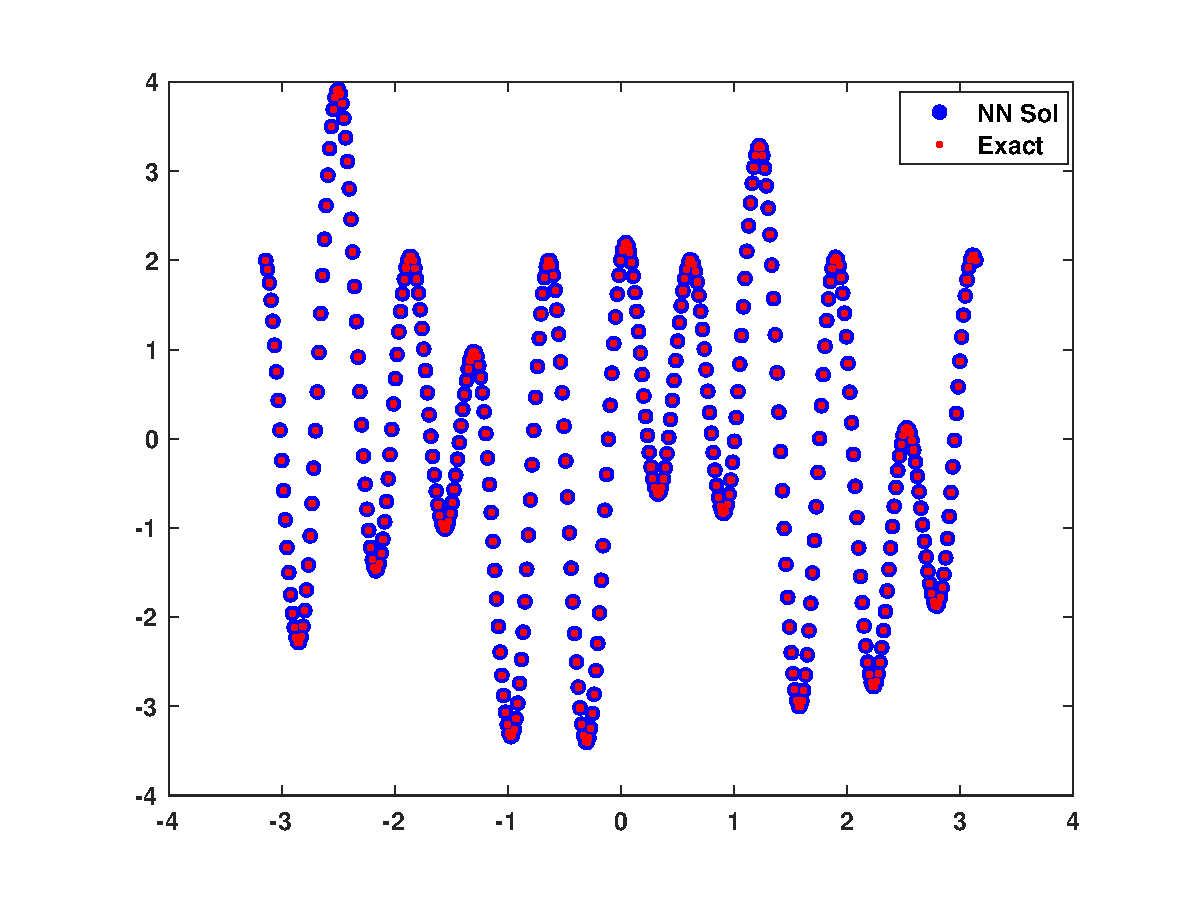
\includegraphics[width=0.5\textwidth]{FNNPer.eps}}
%     \subfigure{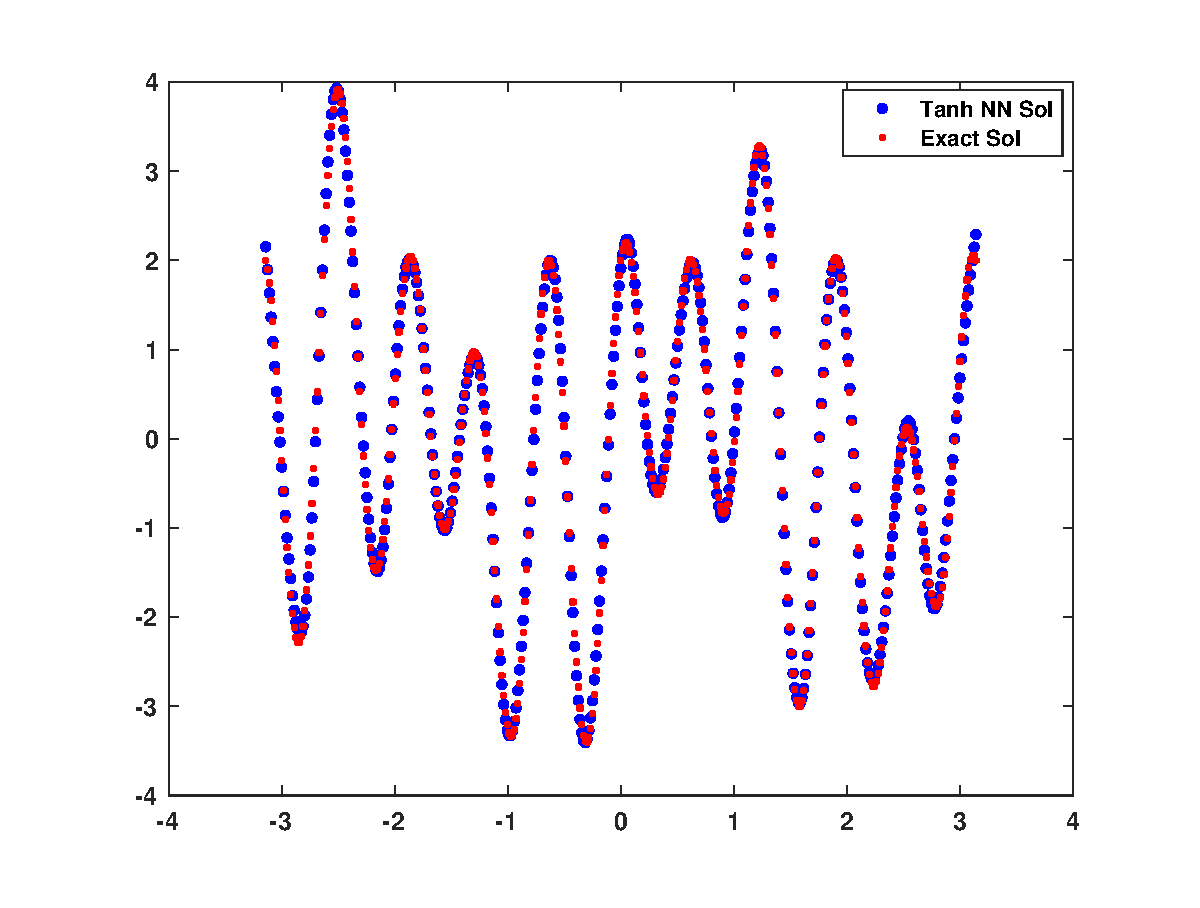
\includegraphics[width=0.5\textwidth]{NNtanhExact.eps}}
%     \caption{(Top)Comparison between the approximation obtained by our Fourier Neural Network and the exact solution. (Bottom)Comparison between the approximation obtained by using a tanh activation function and the exact solution}
%     \label{fig:fourvsNN_per}
% \end{figure}

 
%  \begin{figure}[!htb]
%     \centering
%     \subfigure{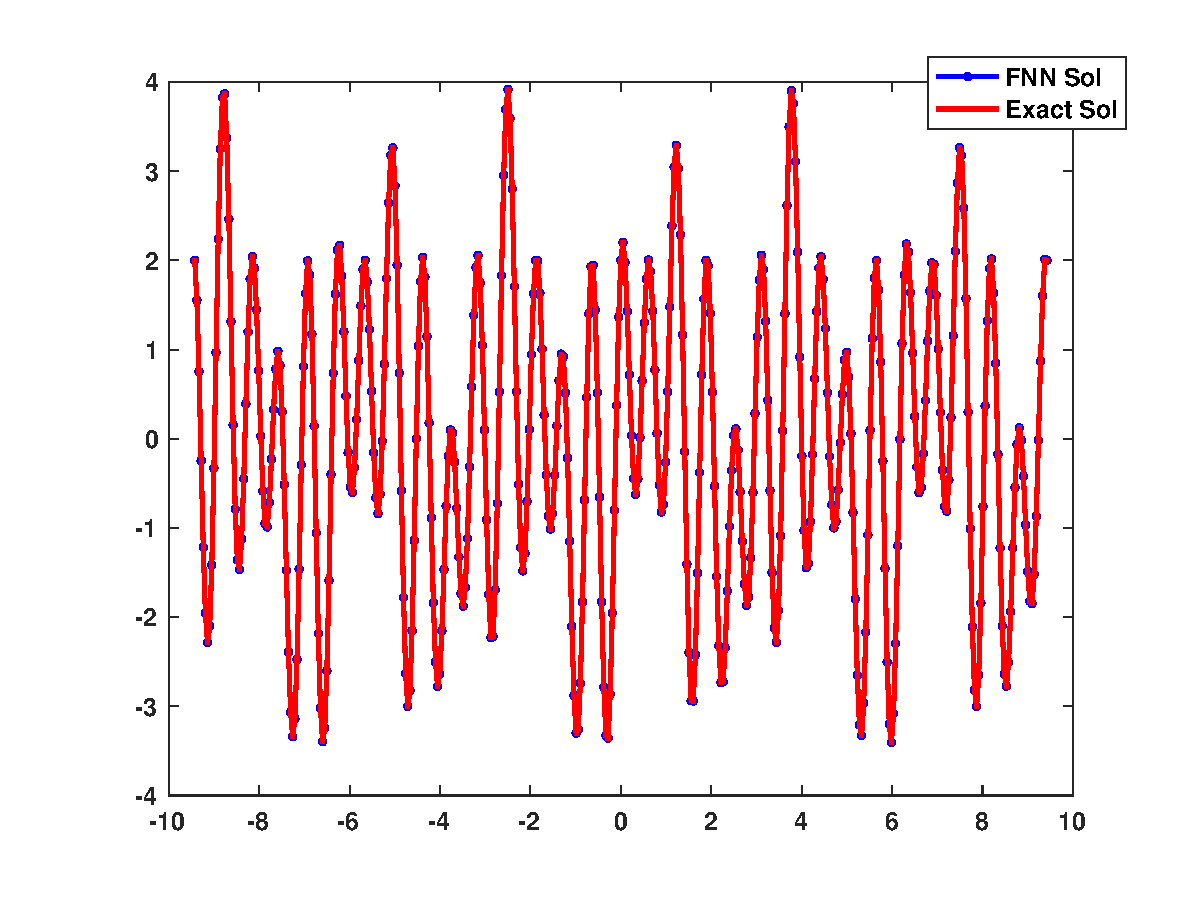
\includegraphics[width=0.5\textwidth]{FNN3pPeri.eps}}
%     \subfigure{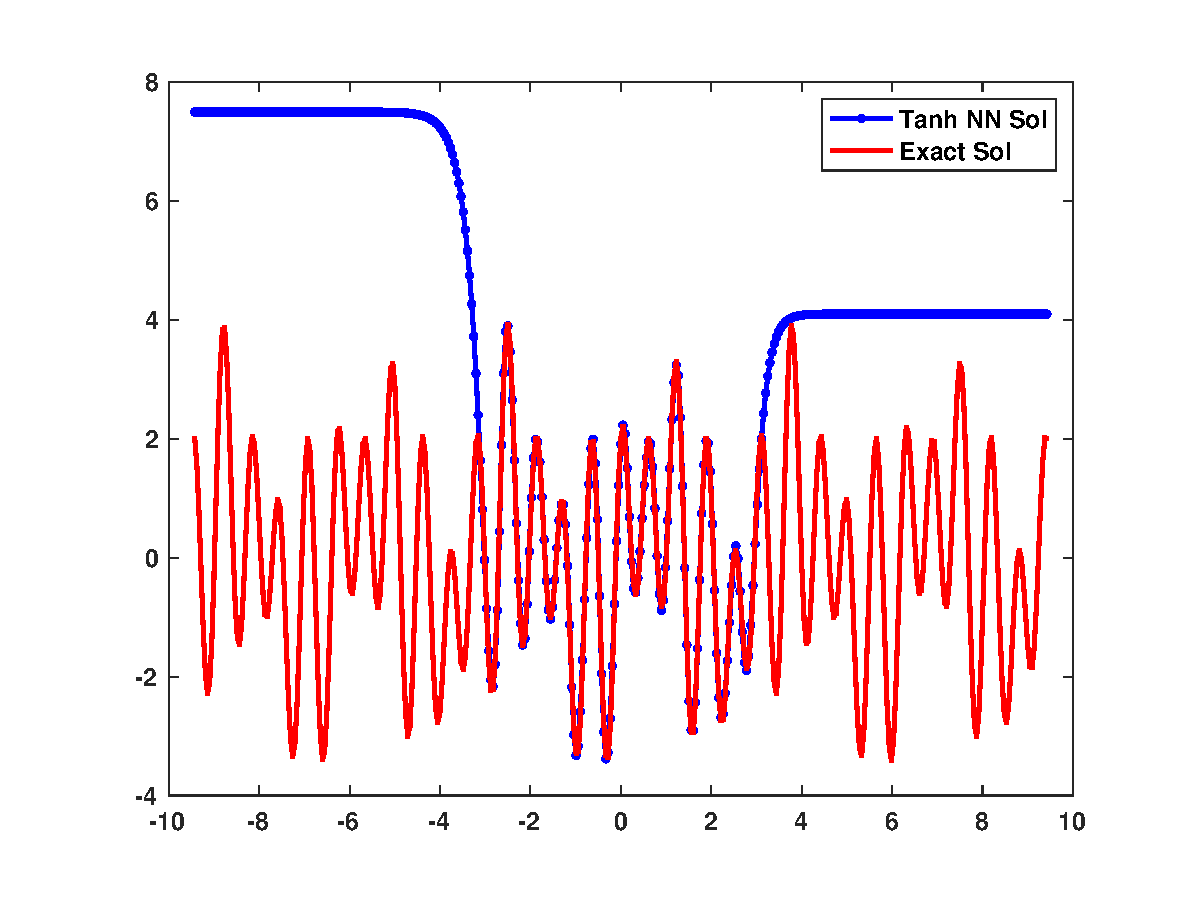
\includegraphics[width=0.5\textwidth]{NNTanh3pi.eps}}
%     \caption{(Top)Comparison between the approximation obtained by our Fourier Neural Network and the exact solution. (Bottom)Comparison between the approximation obtained by using a tanh activation function and the exact solution}
%     \label{fig:fourvsNN_per3pi}
% \end{figure}
%   We can see better in figure (\ref{fig:fourvsNN_per}) that for the same network architecture, our neural network is more accurate. As seen in figures (\ref{fig:fourvsNN_per3pics}) and  (\ref{fig:fourvsNN_per3pi}), one advantage of our model is its ability to fit periodic functions correctly outside of the training interval. This means, as with the Fourier series, we can indeed only represent a $T-$periodic function on $[-T, +T]$ as opposed to a much larger interval.



%%%%%%%%%%%%%proof phase shift


% \begin{equation}\label{fourier_shift_1d}
%     S_N u(x) = \frac{a_0}{2} + \sum_{n=1}^N c_{n} \cos(n \omega x + \psi_{n})
% \end{equation}
% where $c_{n} = \sqrt{a_{n}^2 + b_{n}^2}$ and $\psi_n = \arctan2(-b_{n},a_{n})$. The function $\arctan2$ is defined as follows:
% \begin{equation}
%   \arctan2(y, x) = 
%     \begin{cases}
%       \arctan(y/x) & \text{if $x>0$}\\
%       \arctan(y/x)+\pi & \text{if $x<0$ and $y>0$ }\\
%       \arctan(y/x)-\pi & \text{if $x<0$ and $y<0$ }\\
%       \pi/2 & \text{if $x=0$ and $y>0$ }\\
%       -\pi/2 & \text{if $x=0$ and $y<0$ }\\
%       \pm \infty & \text{if $x=0$ and $y=0$ }
%     \end{cases}       
% \end{equation}
% For simplicity, we suppose $a_n >0$ to show the equivalency of the two forms of the Fourier series. We have, $$c_{n} \cos(n \omega x + \psi_{n}) = c_{n}\left(\cos(n \omega x) \cos(\psi_{n}) - \sin(n \omega x) \sin(\psi_{n})\right)$$
% And, using the fact that $$\cos(\arctan2(-b_{n},a_{n})) = \frac{1}{\sqrt{1+(\frac{b_n}{a_n})^2}}$$
% and
% $$\sin(\arctan2(-b_{n},a_{n})) = \frac{\frac{-b_n}{a_n}}{\sqrt{1+(\frac{b_n}{a_n})^2}}\; ,$$

% we have for $n \geq 1$ 
% \begin{align*}
%     c_{n} \cos(n \omega x + \psi_{n}) &= \sqrt{a_{n}^2 + b_{n}^2}\left(\cos(n \omega x) \frac{1}{\sqrt{1+(\frac{b_n}{a_n})^2}} - \sin(n \omega x) \frac{\frac{-b_n}{a_n}}{\sqrt{1+(\frac{b_n}{a_n})^2}}\right)\\
%   &= \sqrt{a_{n}^2 + b_{n}^2}\left(\cos(n \omega x) \frac{a_n}{\sqrt{a_n^2+b_n^2}} - \sin(n \omega x) \frac{- b_n}{\sqrt{a_n^2+b_n^2}}\right) \\
%   &= a_n\cos(n \omega x) +b_n \sin(n \omega x) \\
% \end{align*}

% We showcase the approximation obtained by our neural network in figure (\ref{Fnnx2})
%   \begin{figure}[!htb]
%     \centering
%     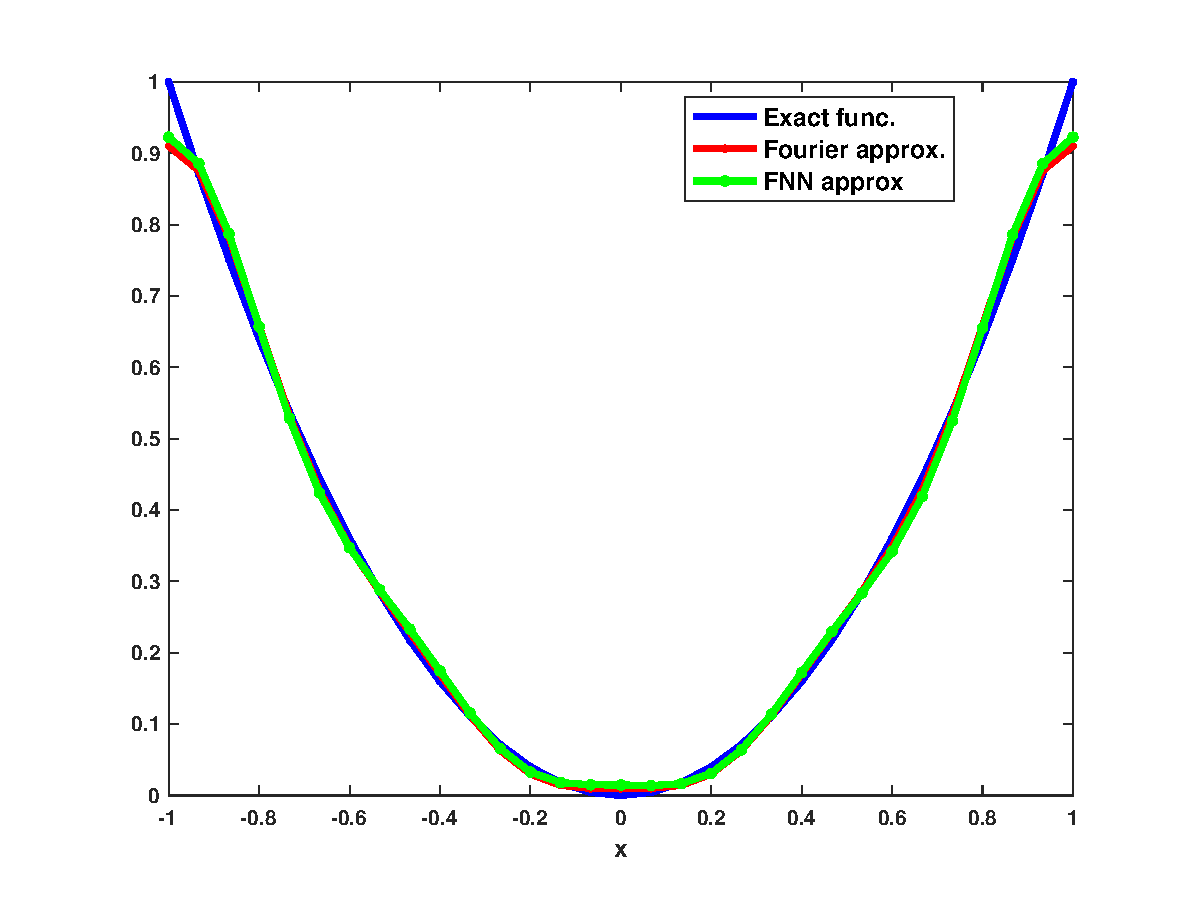
\includegraphics[width=.8\textwidth]{fnnvsfourvsexactx2.eps}
%     \caption{Comparison between $f(x) = x^2$, $S_4 f$ and the output of the FNN}
%     \label{Fnnx2}
% \end{figure}
%  \begin{figure}[!htb]
%     \centering
%     \subfigure{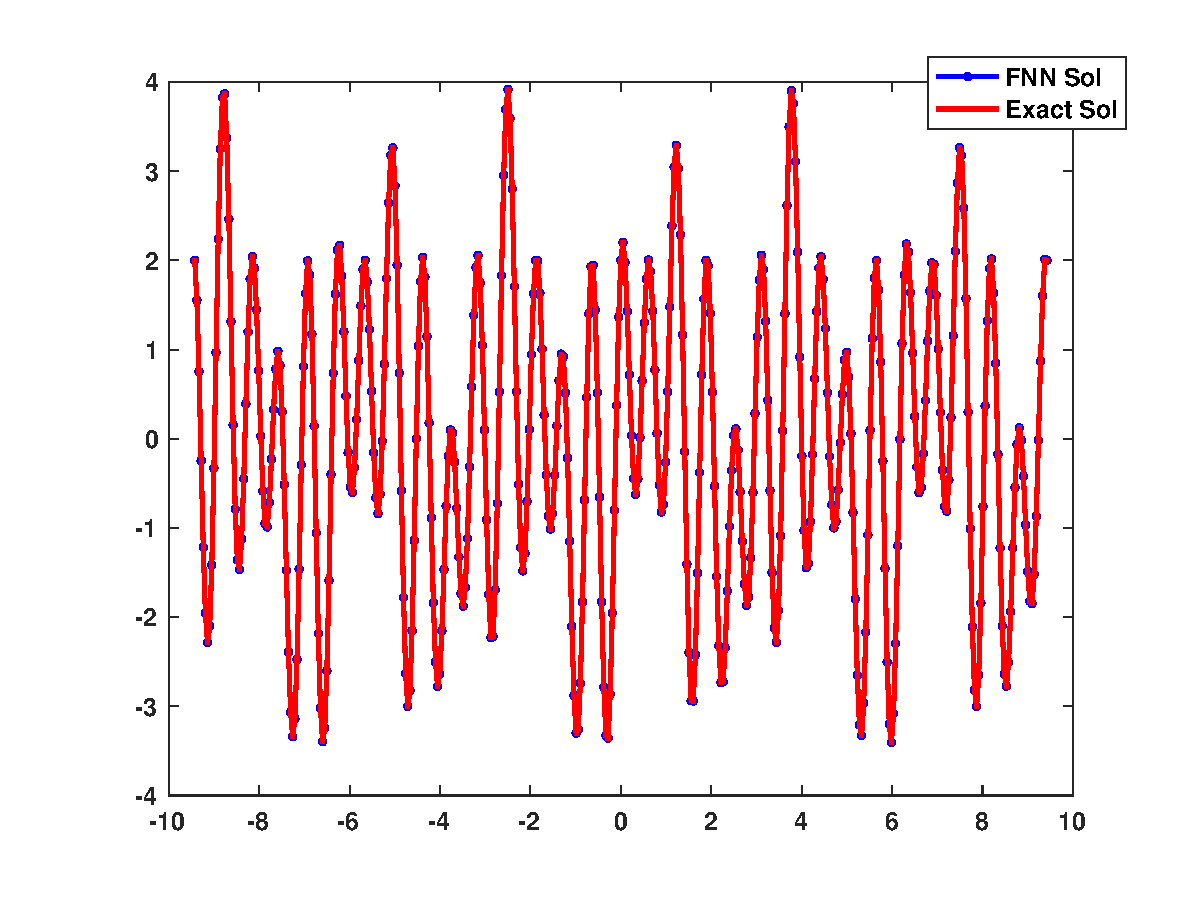
\includegraphics[width=0.5\textwidth]{FNN3pPeri.eps}}
%     \subfigure{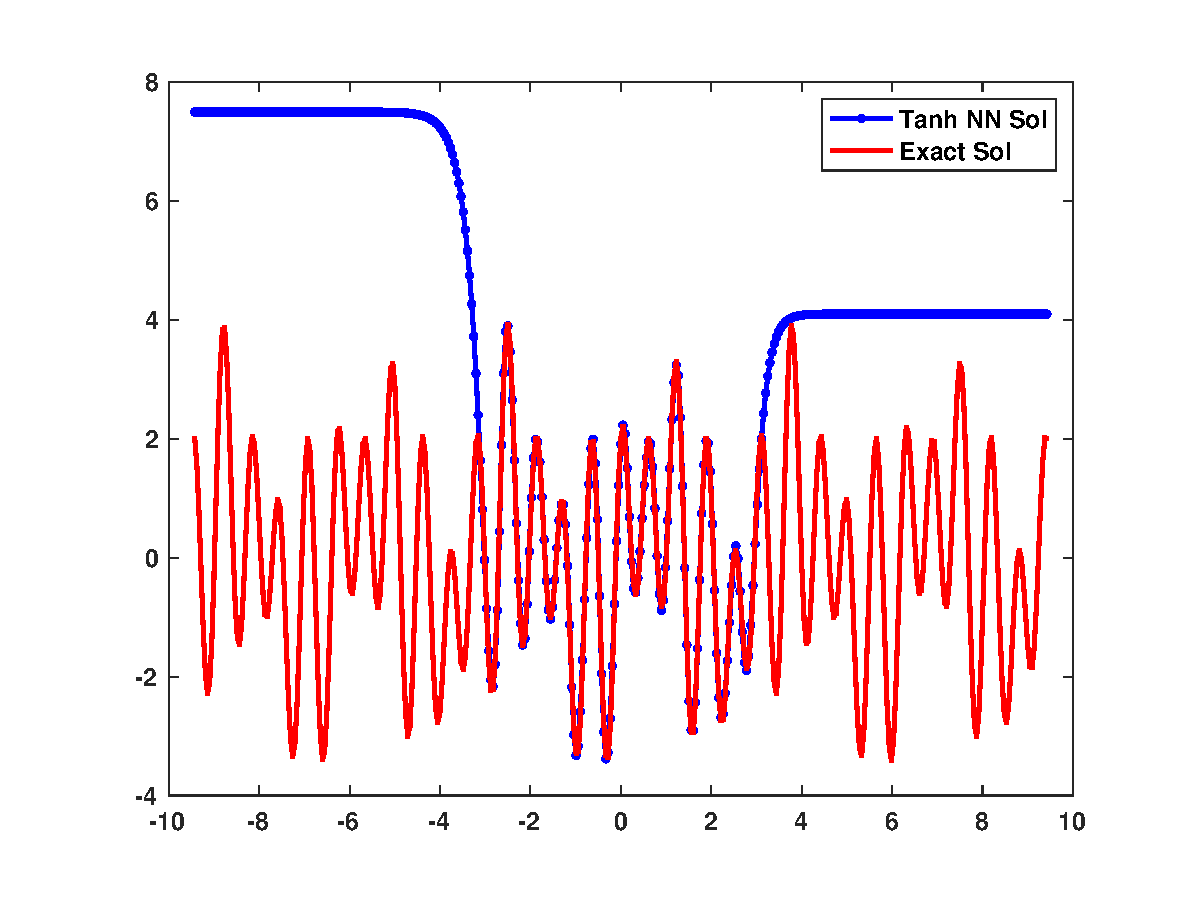
\includegraphics[width=0.5\textwidth]{NNTanh3pi.eps}}
%     \caption{(Top)Comparison between the approximation obtained by our Fourier Neural Network and the exact solution. (Bottom)Comparison between the approximation obtained by using a tanh activation function and the exact solution}
%     \label{fig:fourvsNN_per3pi}
% \end{figure}